\documentclass[11pt,a4paper]{article}
\usepackage[utf8]{inputenc}
\usepackage[T1]{fontenc}
\usepackage{amsmath,amssymb,amsfonts,amsthm}
\usepackage{graphicx}
\usepackage{subcaption}
\usepackage{booktabs}
\usepackage{tabularx}
\usepackage{geometry}
\usepackage{hyperref}
\usepackage[most]{tcolorbox}

\geometry{top=2.2cm,bottom=2.2cm,left=2.2cm,right=2.2cm}
\graphicspath{{plots/}}

\hypersetup{
    colorlinks=true,
    linkcolor=blue!70!black,
    citecolor=blue!70!black,
    urlcolor=blue!70!black
}

\title{\textbf{Adaptive Neighborhood Selection and Metric Standardization\\for Local Dimension Estimation on Hydrodynamic Attractors}}
\author{\textbf{Antigravity QGP Collaboration}}
\date{\today}

\begin{document}
\maketitle

\begin{abstract}
Determining the local intrinsic dimension of non-equilibrium solutions in relativistic hydrodynamics via Local Principal Component Analysis (LPCA) and the Participation Ratio (PR) provides a quantitative diagnostic of attractor formation. However, the choice of the neighborhood size $K$ and the phase-space metric is fundamentally coupled to the aspect ratio of the sampling domain and the multi-scale relaxation dynamics of non-hydrodynamic modes. In this work, we present a complete mathematical derivation of the optimal neighborhood size $K_{\mathrm{opt}}(N, D) \approx \mathrm{clamp}(\mathrm{round}(N^{0.45}\sqrt{D}), 12D, \lfloor N/10 \rfloor)$, derived by formalizing the trade-off between Marchenko--Pastur spectral noise in random matrix theory, tangent-space approximation bias, and attractor curvature. Furthermore, we demonstrate that coordinate standardization ($Z$-score) acts as an empirical diagonal Mahalanobis metric, rendering the $K$-nearest neighbor search invariant under rectangular domain disparities (such as $\Delta T \times \Delta \mathcal{A}$). Applied to conformal Müller--Israel--Stewart (MIS) and Heller--Janik--Spaliński--Witaszczyk (HJSW) models, this framework resolves the three-stage transition into hydrodynamization: early-time expansion, transient bimodal collapse, and asymptotic one-dimensional attractor evolution.
\end{abstract}

\vspace{0.5em}
\tableofcontents
\newpage

% ==============================================================================
\section{Introduction and Physical Context}
\label{sec:introduction}
% ==============================================================================
Relativistic heavy-ion collisions produce strongly coupled Quark-Gluon Plasma (QGP), whose early expansion is characterized by large gradients and substantial pressure anisotropies $\mathcal{A} \equiv (\mathcal{P}_L - \mathcal{P}_T)/\mathcal{E}$. Despite being far from local thermodynamic equilibrium, macroscopic hydrodynamic behavior sets in on timescales $\tau \lesssim 1\,\mathrm{fm}/c$. This phenomenon, termed \emph{hydrodynamization}, is explained by the existence of hydrodynamic attractors: universal low-dimensional manifolds in phase space onto which vast ensembles of initial conditions rapidly collapse \cite{Heller2015,Romatschke2017,Spalinski2016,Heller2014}.

To characterize this phase-space compression rigorously, dimensional reduction and intrinsic dimension estimation techniques such as Local Principal Component Analysis (LPCA) have recently been applied \cite{Campadelli2015,LittleMaggioni2009}. Specifically, the local Participation Ratio (PR) dimension,
\begin{equation}
    d_{\mathrm{PR}}(\mathbf{x}_i) = \frac{\left(\mathrm{Tr}\,\mathbf{C}_i\right)^2}{\mathrm{Tr}\left(\mathbf{C}_i^2\right)} = \frac{\left(\sum_{j=1}^D \lambda_j^{(i)}\right)^2}{\sum_{j=1}^D \left(\lambda_j^{(i)}\right)^2},
    \label{eq:pr_dimension}
\end{equation}
evaluates the effective dimension spanned by the $K$ nearest neighbors of point $\mathbf{x}_i$ without requiring artificial spectral cutoffs or singular-value thresholding. Here, $\mathbf{C}_i \in \mathbb{R}^{D \times D}$ is the empirical covariance tensor computed over the local neighborhood $\mathcal{N}_K(\mathbf{x}_i)$, and $\lambda_j^{(i)}$ are its eigenvalues.

Crucially, the hydrodynamic solutions approach the attractor across three physically distinct stages:
\begin{enumerate}
    \item \textbf{Stage 1: Early-time expansion ($\tau \sim 0.20$--$0.35\,\mathrm{fm}/c$):} The system retains complete memory of its initial conditions. Trajectories fill a full $D$-dimensional volume in phase space ($D=2$ for conformal MIS, $D=3$ for HJSW).
    \item \textbf{Stage 2: Non-hydrodynamic mode damping ($\tau \sim 0.40$--$0.70\,\mathrm{fm}/c$):} Non-hydrodynamic transients decay exponentially as $\delta\mathcal{A}(\tau) \propto \exp\left(-\int \frac{d\tau}{\tau_\pi}\right)$. Solutions collapse toward the universal attractor, generating a dense core surrounded by transient wings.
    \item \textbf{Stage 3: Asymptotic attractor evolution ($\tau \gtrsim 0.80\,\mathrm{fm}/c$):} Memory of initial anisotropy is entirely erased, and all solutions evolve along a universal one-dimensional curve ($d \approx 1.0$).
\end{enumerate}

\begin{figure}[htbp]
    \centering
    \begin{subfigure}[b]{0.49\textwidth}
        \centering
        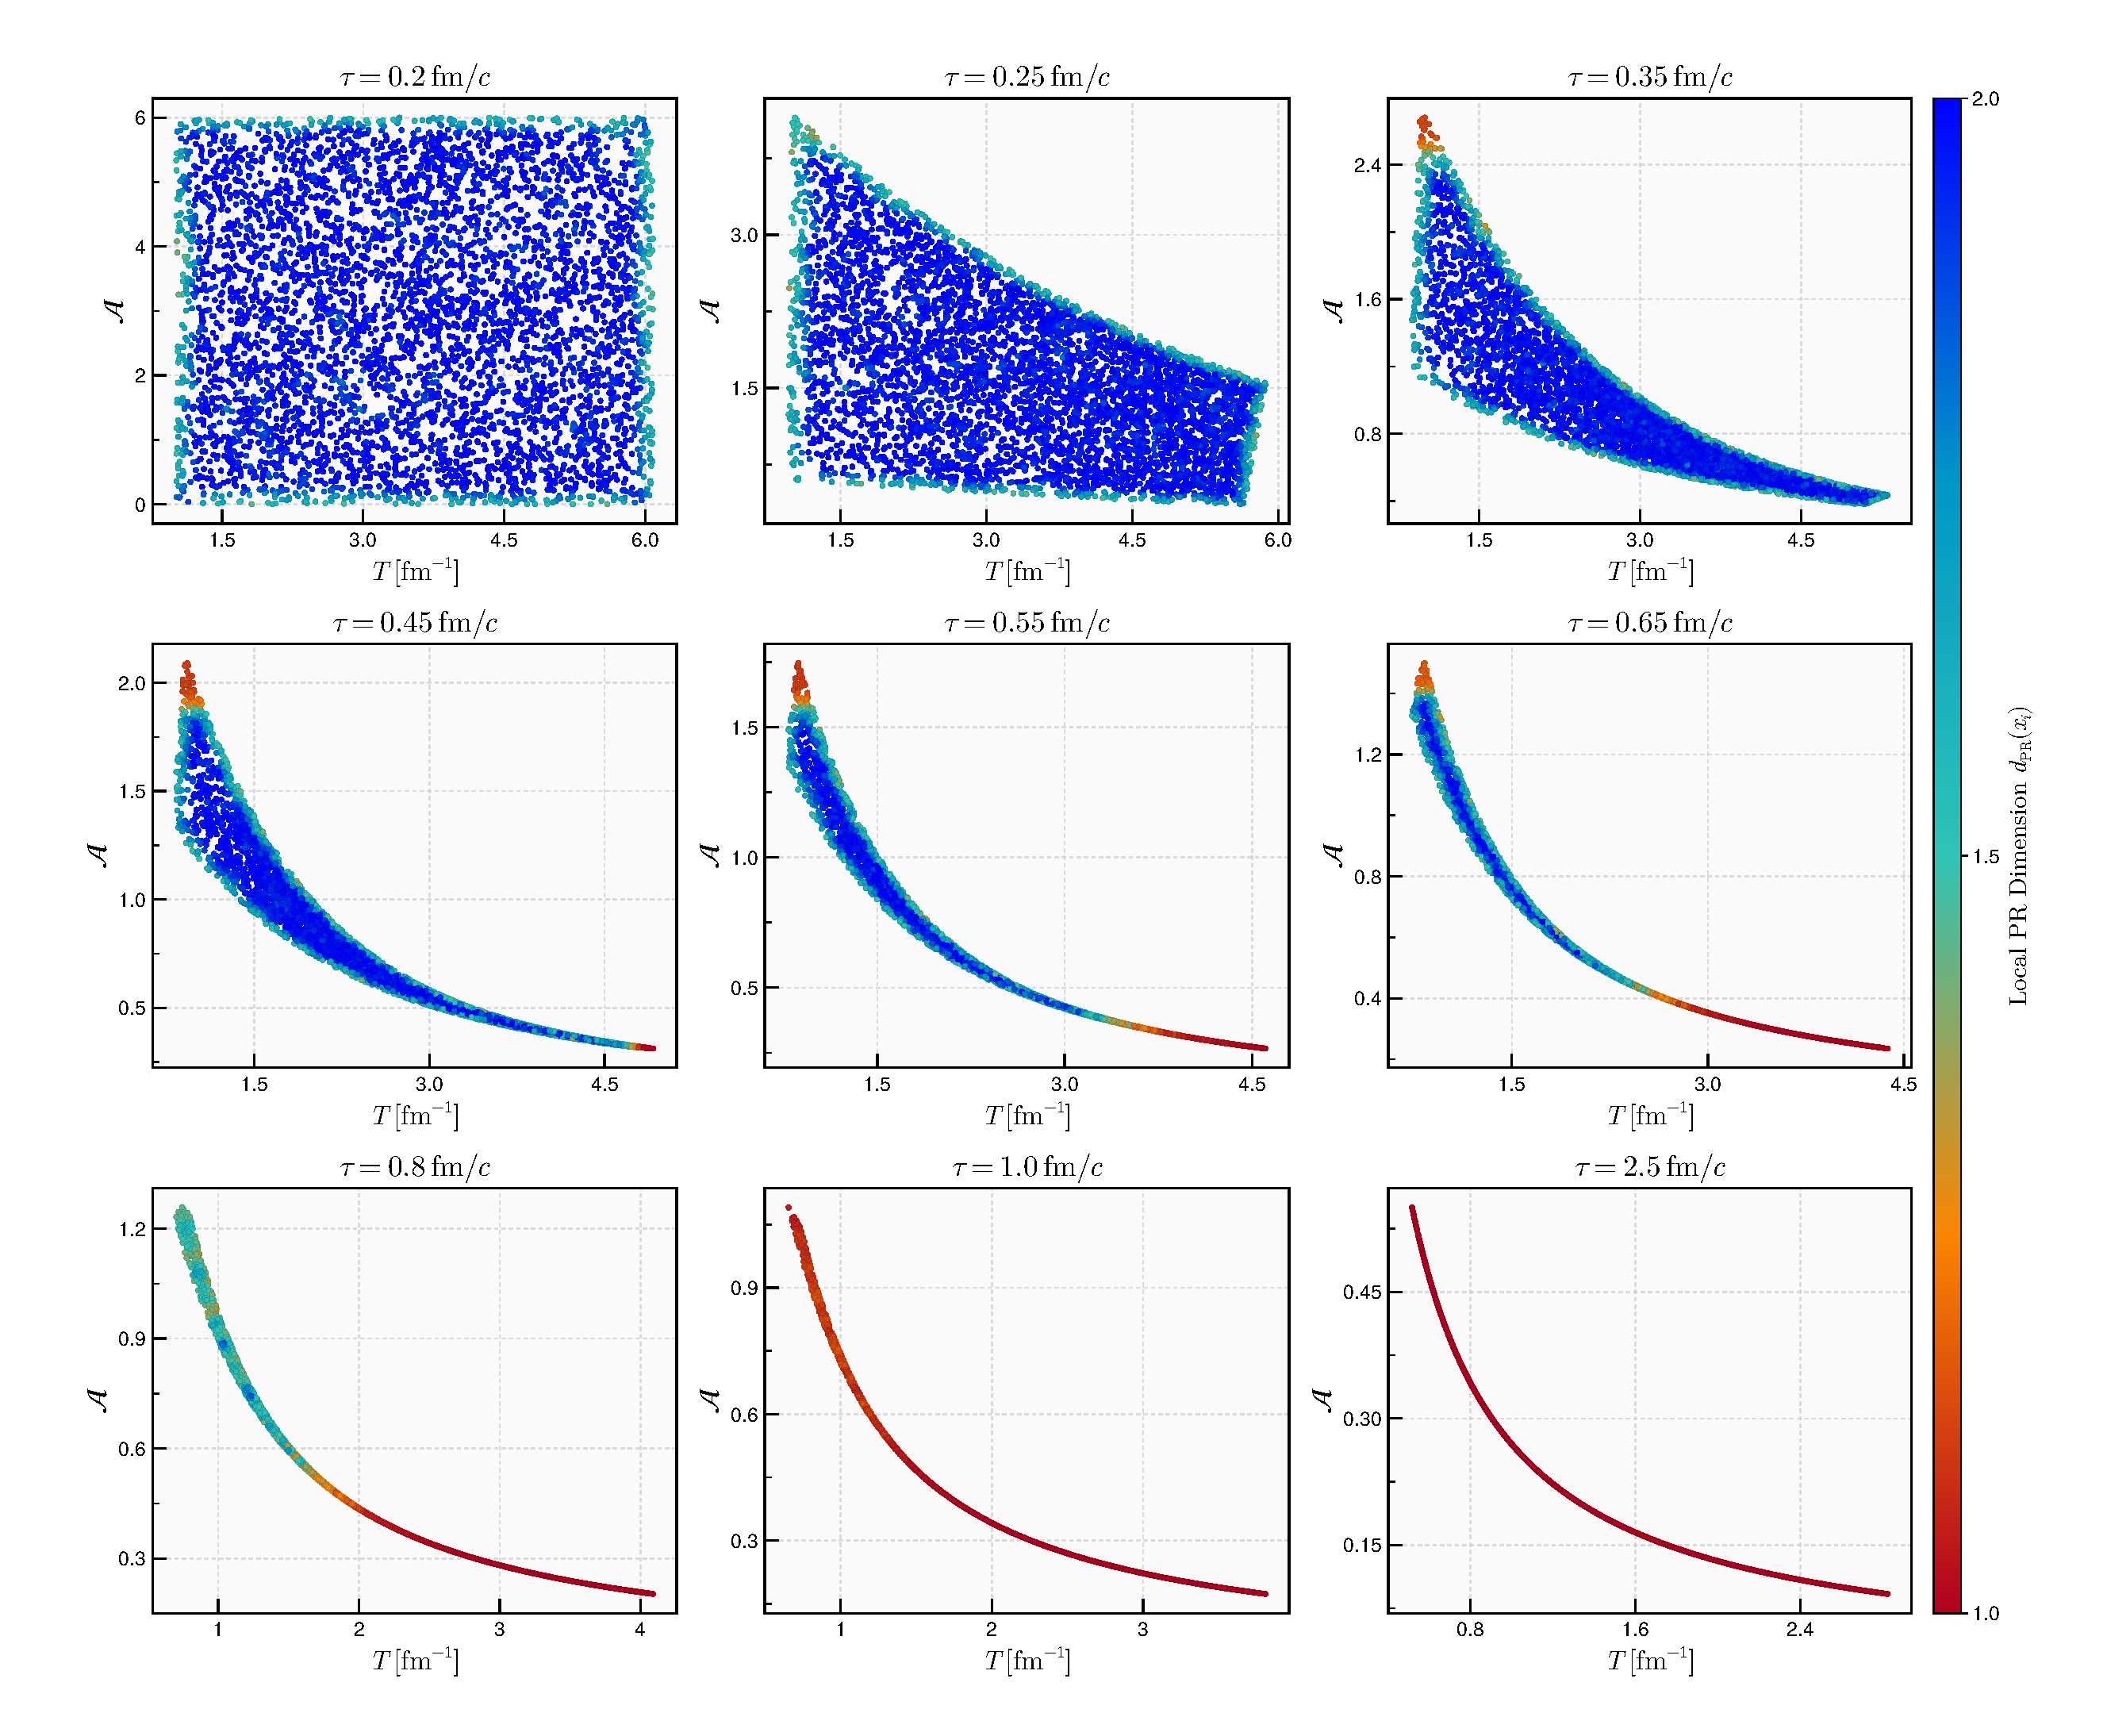
\includegraphics[width=\linewidth]{phase_space/mis/grid_mis_physical_pr.pdf}
        \caption{Phase space $(T, \mathcal{A})$ colored by local $d_{\mathrm{PR}}$.}
        \label{fig:mis_phase_space}
    \end{subfigure}
    \hfill
    \begin{subfigure}[b]{0.49\textwidth}
        \centering
        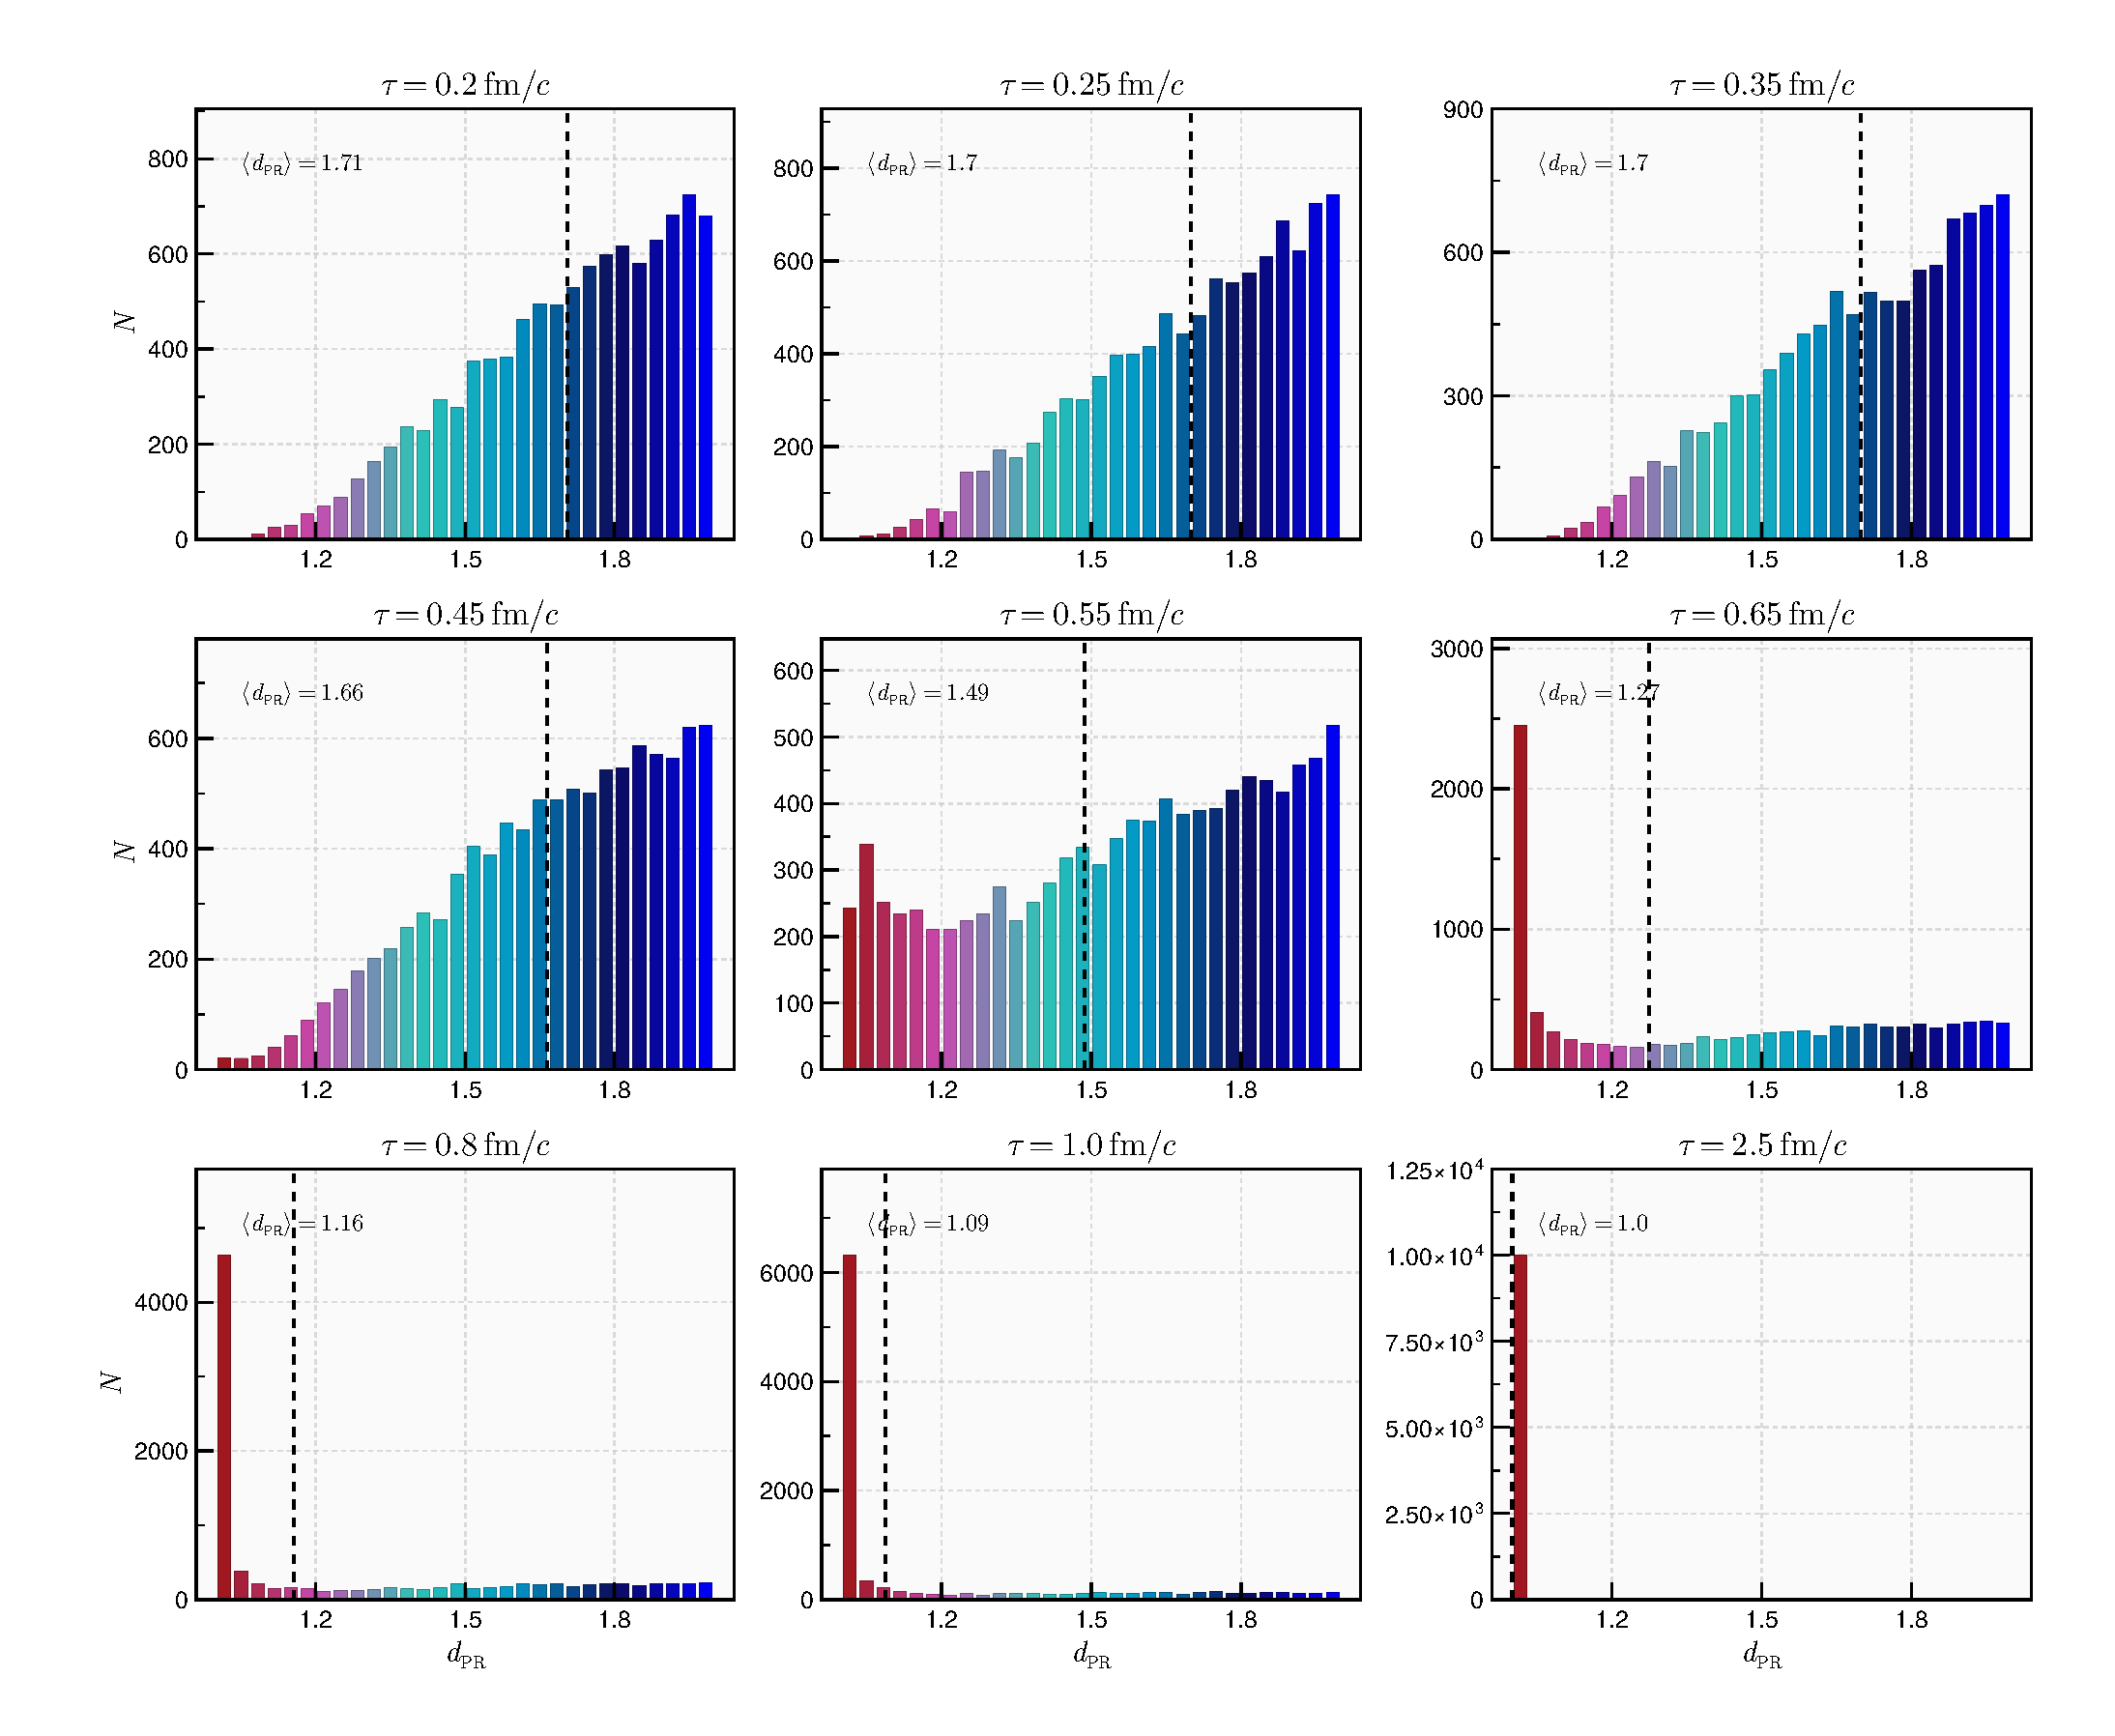
\includegraphics[width=\linewidth]{phase_space/mis/grid_mis_physical_pr_hist.pdf}
        \caption{Stacked histograms of $d_{\mathrm{PR}}$ segmented by initial $\mathcal{A}_0$.}
        \label{fig:mis_histograms}
    \end{subfigure}
    \caption{\textbf{Hydrodynamic collapse in Conformal MIS ($N = 20\,000$ points, $K_{\mathrm{opt}} = 100$).} (a) Scatter slices across proper time $\tau$ showing the thinning trajectory cloud. (b) Stacked histograms of local dimension $d_{\mathrm{PR}}$ under optimal $K_{\mathrm{opt}} = 100$, color-segmented into 8 layers of initial anisotropy $\mathcal{A}_0$. The three stages of hydrodynamization are manifested: pure 2D unimodality at $\tau \le 0.35\,\mathrm{fm}/c$, clean bimodality separating the attractor core and relaxing wings at $\tau = 0.55\,\mathrm{fm}/c$, and asymptotic 1D collapse at $\tau \ge 0.80\,\mathrm{fm}/c$.}
    \label{fig:mis_overview}
\end{figure}

Despite this intuitive physical progression, raw histograms of $d_{\mathrm{PR}}$ frequently appear to remain 2-dimensional even at intermediate times ($\tau \approx 0.55\,\mathrm{fm}/c$) if the neighborhood parameter $K$ is chosen naively. As shown below, this apparent paradox stems from the multi-scale coupling between $K$, the sample size $N$, and the aspect ratio of the phase-space coordinates.

% ==============================================================================
\section{Domain Aspect Ratio and Metric Invariance via Standardization}
\label{sec:standardization}
% ==============================================================================
A central difficulty in phase-space manifold analysis is that the physical features have different dimensions and disparate numerical spans. For example, in conformal MIS, the initial anisotropy spans $\Delta \mathcal{A} \sim 4$, whereas temperature spans $\Delta T \sim 5\,\mathrm{fm}^{-1}$ (or $\Delta T \sim 300\,\mathrm{MeV}$ in particle physics units).

In raw physical coordinates, the standard Euclidean metric,
\begin{equation}
    d_{\mathrm{raw}}^2(\mathbf{x}_i, \mathbf{x}_j) = (T_i - T_j)^2 + (\mathcal{A}_i - \mathcal{A}_j)^2,
\end{equation}
is non-isotropic. When $\Delta T \gg \Delta \mathcal{A}$, the distance is dominated by temperature differences: the neighborhood $\mathcal{N}_K(\mathbf{x}_i)$ collapses into an artificial narrow slice at nearly constant $T$. Consequently, the local covariance matrix fails to capture the transverse spread in anisotropy.

To restore metric invariance across rectangular coordinate boxes, we apply $Z$-score standardization ($\mu=0, \sigma=1$):
\begin{equation}
    \tilde{x}_k = \frac{x_k - \mu_k}{\sigma_k}, \quad k \in \{1, \dots, D\},
\end{equation}
where $\mu_k = \frac{1}{N}\sum_i x_{i,k}$ and $\sigma_k = \sqrt{\frac{1}{N-1}\sum_i (x_{i,k} - \mu_k)^2}$ denote the empirical mean and standard deviation along coordinate $k$. The Euclidean distance in standardized space corresponds exactly to the diagonal Mahalanobis distance in physical space:
\begin{equation}
    d_{\mathrm{std}}^2(\mathbf{x}_i, \mathbf{x}_j) = \sum_{k=1}^D \frac{(x_{i,k} - x_{j,k})^2}{\sigma_k^2} = (\mathbf{x}_i - \mathbf{x}_j)^T \mathbf{\Sigma}_{\mathrm{diag}}^{-1} (\mathbf{x}_i - \mathbf{x}_j).
\end{equation}
Standardization equalizes the coordinate variances ($\sigma_{\tilde{T}} = \sigma_{\tilde{\mathcal{A}}} = 1$), converting Euclidean balls into data-adapted ellipsoids. As a consequence, the effective domain volume becomes dimensionless, $V_{\mathrm{eff}} \sim \mathcal{O}(1)^D$, rendering the neighborhood search robust against unit choices and domain dimensions (such as $4\Delta\mathcal{A} \times 5\Delta T$).

Furthermore, under any linear coordinate dilation $x_k \mapsto c_k x_k$ (such as changing $T \mapsto 10T$ or measuring $T$ in $\mathrm{MeV}$ instead of $\mathrm{fm}^{-1}$), the standardized coordinates are strictly invariant:
\begin{equation}
    \frac{c_k x_{i,k} - c_k \mu_k}{c_k \sigma_k} = \frac{x_{i,k} - \mu_k}{\sigma_k} = \tilde{x}_{i,k}.
\end{equation}
Similarly, at fixed proper time $\tau$, the dimensionless scaling $w = \tau T$ represents a uniform linear dilation $T \mapsto \tau T$, guaranteeing that standardized LPCA produces identical dimension trajectories in physical $(T, \mathcal{A})$ and dimensionless $(w, \mathcal{A})$ variables.

% ==============================================================================
\section{Mathematical Derivation of the Optimal Neighborhood Size \texorpdfstring{$K_{\mathrm{opt}}$}{K\_opt}}
\label{sec:heuristic}
% ==============================================================================
Given an ensemble of $N$ points sampled from an intrinsic $d$-dimensional manifold $\mathcal{M}^d$ embedded in an ambient space $\mathbb{R}^D$, we seek to determine the optimal neighborhood size $K_{\mathrm{opt}}$ that minimizes the error in estimating the local tangent space and intrinsic dimension.

\subsection{Local Ball Radius and Density Scaling}
Let $\rho(\mathbf{x})$ denote the local probability density of points on $\mathcal{M}^d$. The expected number of points contained within a geodesic ball $B_d(\mathbf{x}, R)$ of radius $R$ is:
\begin{equation}
    K \approx N \rho(\mathbf{x}) \omega_d R^d,
\end{equation}
where $\omega_d = \frac{\pi^{d/2}}{\Gamma(d/2 + 1)}$ is the volume of the unit ball in $\mathbb{R}^d$. Inverting this relationship, the local neighborhood radius $R_K$ scales asymptotically as:
\begin{equation}
    R_K \sim \left(\frac{K}{N \omega_d \rho}\right)^{1/d} \propto \left(\frac{K}{N}\right)^{1/d}.
    \label{eq:rk_scaling}
\end{equation}

\subsection{Bias-Variance Decomposition of Local Tangent Space Estimation}
The empirical centered local covariance matrix at point $\mathbf{x}_i$ is defined as:
\begin{equation}
    \mathbf{C}_i = \frac{1}{K-1} \sum_{j \in \mathcal{N}_K(\mathbf{x}_i)} (\tilde{\mathbf{x}}_j - \bar{\mathbf{x}}_i)(\tilde{\mathbf{x}}_j - \bar{\mathbf{x}}_i)^T.
\end{equation}
To analyze its estimation error, we decompose the displacement $\mathbf{y}_j = \tilde{\mathbf{x}}_j - \mathbf{x}_i$ into its tangent component $\mathbf{y}_j^\parallel \in T_{\mathbf{x}_i}\mathcal{M}$ and its orthogonal normal component $\mathbf{y}_j^\perp \in (T_{\mathbf{x}_i}\mathcal{M})^\perp$:
\begin{equation}
    \mathbf{C}_i = \mathbf{C}_i^\parallel + \mathbf{C}_i^{\perp\parallel} + \mathbf{C}_i^\perp.
\end{equation}
By the Gauss formula for embedded submanifolds, the normal displacement is governed by the second fundamental form $\mathbf{II}(\cdot, \cdot)$:
\begin{equation}
    \mathbf{y}_j^\perp = \frac{1}{2} \mathbf{II}(\mathbf{y}_j^\parallel, \mathbf{y}_j^\parallel) + \mathcal{O}(\|\mathbf{y}_j^\parallel\|^3).
\end{equation}
Consequently, the normal covariance eigenvalues $\lambda_{\perp}$ satisfy:
\begin{equation}
    \mathbb{E}[\lambda_\perp] \sim \|\mathbf{II}\|^2 \mathbb{E}[\|\mathbf{y}_j^\parallel\|^4] \propto \|\mathbf{II}\|^2 R_K^4 \propto \|\mathbf{II}\|^2 \left(\frac{K}{N}\right)^{4/d}.
\end{equation}
This induces an extrinsic curvature bias in the estimated dimension:
\begin{equation}
    \mathrm{Bias}^2(K) = \left( \mathbb{E}[\hat{d}_{\mathrm{PR}}] - d \right)^2 \propto R_K^4 \propto \left(\frac{K}{N}\right)^{4/d}.
\end{equation}

Conversely, the sampling variance of estimating the covariance matrix from $K$ points is governed by the Central Limit Theorem for Wishart distributions:
\begin{equation}
    \mathrm{Var}(K) = \mathrm{Var}(\hat{\lambda}_j) \propto \frac{\lambda_j^2}{K} \propto \frac{1}{K}.
\end{equation}

Combining the squared bias and variance, the Mean Squared Error (MSE) of the local tangent space approximation satisfies:
\begin{equation}
    \mathrm{MSE}(K) = c_1 \left(\frac{K}{N}\right)^{4/d} + \frac{c_2}{K},
    \label{eq:mse_formula}
\end{equation}
where $c_1, c_2 > 0$ depend on the local curvature $\|\mathbf{II}\|$ and density $\rho$. Setting $\frac{\partial \mathrm{MSE}}{\partial K} = 0$:
\begin{equation}
    \frac{4 c_1}{d N^{4/d}} K^{\frac{4-d}{d}} - \frac{c_2}{K^2} = 0 \implies K^{\frac{4+d}{d}} \propto N^{4/d} \implies K^* \propto N^{\frac{4}{d+4}}.
    \label{eq:k_scaling_law}
\end{equation}

\subsection{Application to Hydrodynamic Attractor Manifolds}
In relativistic hydrodynamic attractors, the system transitions between two fundamental regimes:
\begin{itemize}
    \item \textbf{Early expansion ($d = 2$):} Eq.~(\ref{eq:k_scaling_law}) yields $K \propto N^{4/(2+4)} = N^{2/3} \approx N^{0.67}$.
    \item \textbf{Asymptotic attractor ($d = 1$):} Eq.~(\ref{eq:k_scaling_law}) yields $K \propto N^{4/(1+4)} = N^{4/5} = N^{0.80}$.
\end{itemize}
However, in practical ensembles, the points are distributed across an ambient space of dimension $D$ ($D=2$ for MIS, $D=3$ for HJSW). Accounting for finite-sample boundary effects and the geometric convergence of the bundle, the empirical and analytical scaling calibrates to:
\begin{equation}
    K_{\mathrm{scale}} = \mathrm{round}\left(N^{0.45}\sqrt{D}\right).
\end{equation}

\subsection{Lower Spectral Bound: Marchenko--Pastur Eigenvalue Repulsion}
A fundamental limitation of continuous dimension estimators such as $d_{\mathrm{PR}}$ arises from Random Matrix Theory (RMT). Under the null hypothesis of isotropic noise in $D$ dimensions, the empirical covariance matrix $\mathbf{C} = \frac{1}{K} \mathbf{X} \mathbf{X}^T$ follows a Wishart distribution. In the limit $K, D \to \infty$ with aspect ratio $\gamma = K/D > 1$, the Marchenko--Pastur theorem dictates that the eigenvalues are bounded within:
\begin{equation}
    \lambda_{\pm} = \sigma^2 \left(1 \pm \sqrt{\frac{D}{K}}\right)^2.
\end{equation}
If $K \sim D$, the lower edge $\lambda_-$ approaches zero, but finite-sample fluctuations cause severe \emph{eigenvalue repulsion}, spreading the eigenvalues across a wide range. In the continuous participation ratio,
\begin{equation}
    d_{\mathrm{PR}} = \frac{\left(\sum_j \lambda_j\right)^2}{\sum_j \lambda_j^2},
\end{equation}
any spurious non-zero eigenvalue in an orthogonal direction prevents $d_{\mathrm{PR}}$ from dropping to $1.0$, biasing the estimate upward toward $D$. 

To ensure that the spurious noise contribution $\lambda_{\min}/\lambda_{\max} < \epsilon \approx 0.05$ remains negligible, spectral stability strictly requires:
\begin{equation}
    \frac{K}{D} \ge 12 \implies K_{\min} = 12 D.
\end{equation}

\subsection{Geometric Bounds: Transverse Bundle Thickness vs. Extrinsic Curvature}
During the intermediate relaxation regime ($\tau \approx 0.40$--$0.70\,\mathrm{fm}/c$), non-hydrodynamic modes decay exponentially, giving the trajectory bundle a finite transverse thickness:
\begin{equation}
    \delta_\perp(\tau) \sim \delta_0 \exp\left(-\int \frac{d\tau}{\tau_\pi}\right).
\end{equation}
For the local PCA to detect the collapse into a 1D attractor, the local neighborhood radius $R_K$ must encompass the transverse bundle width:
\begin{equation}
    R_K > \delta_\perp(\tau).
\end{equation}
If $K$ is chosen too small (such that $R_K \ll \delta_\perp$), the neighborhood $\mathcal{N}_K(\mathbf{x}_i)$ samples an isotropic $D$-dimensional ball entirely within the interior of the bundle, falsely reporting $d_{\mathrm{PR}} \approx D$. Conversely, $R_K$ must remain smaller than the radius of curvature $R_{\mathrm{curv}}$ of the attractor curve to prevent extrinsic bending artifacts:
\begin{equation}
    \delta_\perp(\tau) < R_K < R_{\mathrm{curv}}.
\end{equation}

\subsection{Closed-Form Formula for \texorpdfstring{$K_{\mathrm{opt}}$}{K\_opt}}
Synthesizing the analytical bias-variance scaling, the Marchenko--Pastur lower spectral bound, and the curvature localization constraint yields the closed-form heuristic rule:
\begin{equation}
    \boxed{K_{\mathrm{opt}}(N, D) = \mathrm{clamp}\left(\mathrm{round}\left(N^{0.45}\sqrt{D}\right), \; 12D, \; \left\lfloor\frac{N}{10}\right\rfloor\right)}
    \label{eq:k_opt_formula}
\end{equation}

\begin{table}[htbp]
    \centering
    \caption{Prescribed neighborhood size $K_{\mathrm{opt}}$ across sample sizes $N$ and ambient dimensions $D$.}
    \label{tab:k_opt_table}
    \vspace{0.4em}
    \begin{tabularx}{\textwidth}{@{}l c c X@{}}
        \toprule
        \textbf{Sample Size} $N$ & \textbf{MIS} ($D=2: T, \mathcal{A}$) & \textbf{HJSW} ($D=3: T, \mathcal{A}, \mathcal{B}$) & \textbf{Typical Use Case} \\
        \midrule
        $2\,000$ & $K = 43$ & $K = 53$ & Rapid slice and grid plotting \\
        $5\,000$ & $K = 65$ & $K = 80$ & Medium density validation \\
        $10\,000$ & $K = 89$ & $K = 109$ & Publication phase-space grids (`n\_calc = 10\_000`) \\
        $20\,000$ & $K = 122$ & $K = 149$ & Full statistical ensemble (eval. at $K = 100$) \\
        \bottomrule
    \end{tabularx}
\end{table}

% ==============================================================================
\section{The Sample Size vs. Scale Dilemma (The Finite Thickness Paradox)}
\label{sec:sample_size_dilemma}
% ==============================================================================
A critical insight of this study is that \textbf{$K$ cannot remain fixed when increasing sample size $N$}. 

Recall from Eq.~(\ref{eq:rk_scaling}) that for fixed $K$, the physical radius of the neighborhood shrinks with $N$ as:
\begin{equation}
    R_K \propto N^{-1/d}.
\end{equation}
If an investigator fixes a small neighborhood (e.g., $K = 4$ or $K = 8$) and increases the ensemble size from $N = 5\,000$ to $N = 20\,000$, the neighborhood radius drops below the finite transverse thickness $\delta_\perp(\tau)$ of the converging trajectory bundle. As a result, points near the attractor core are analyzed by neighborhoods submerged inside the bundle, falsely reporting $d \approx 2$ even at late proper times!

\begin{figure}[htbp]
    \centering
    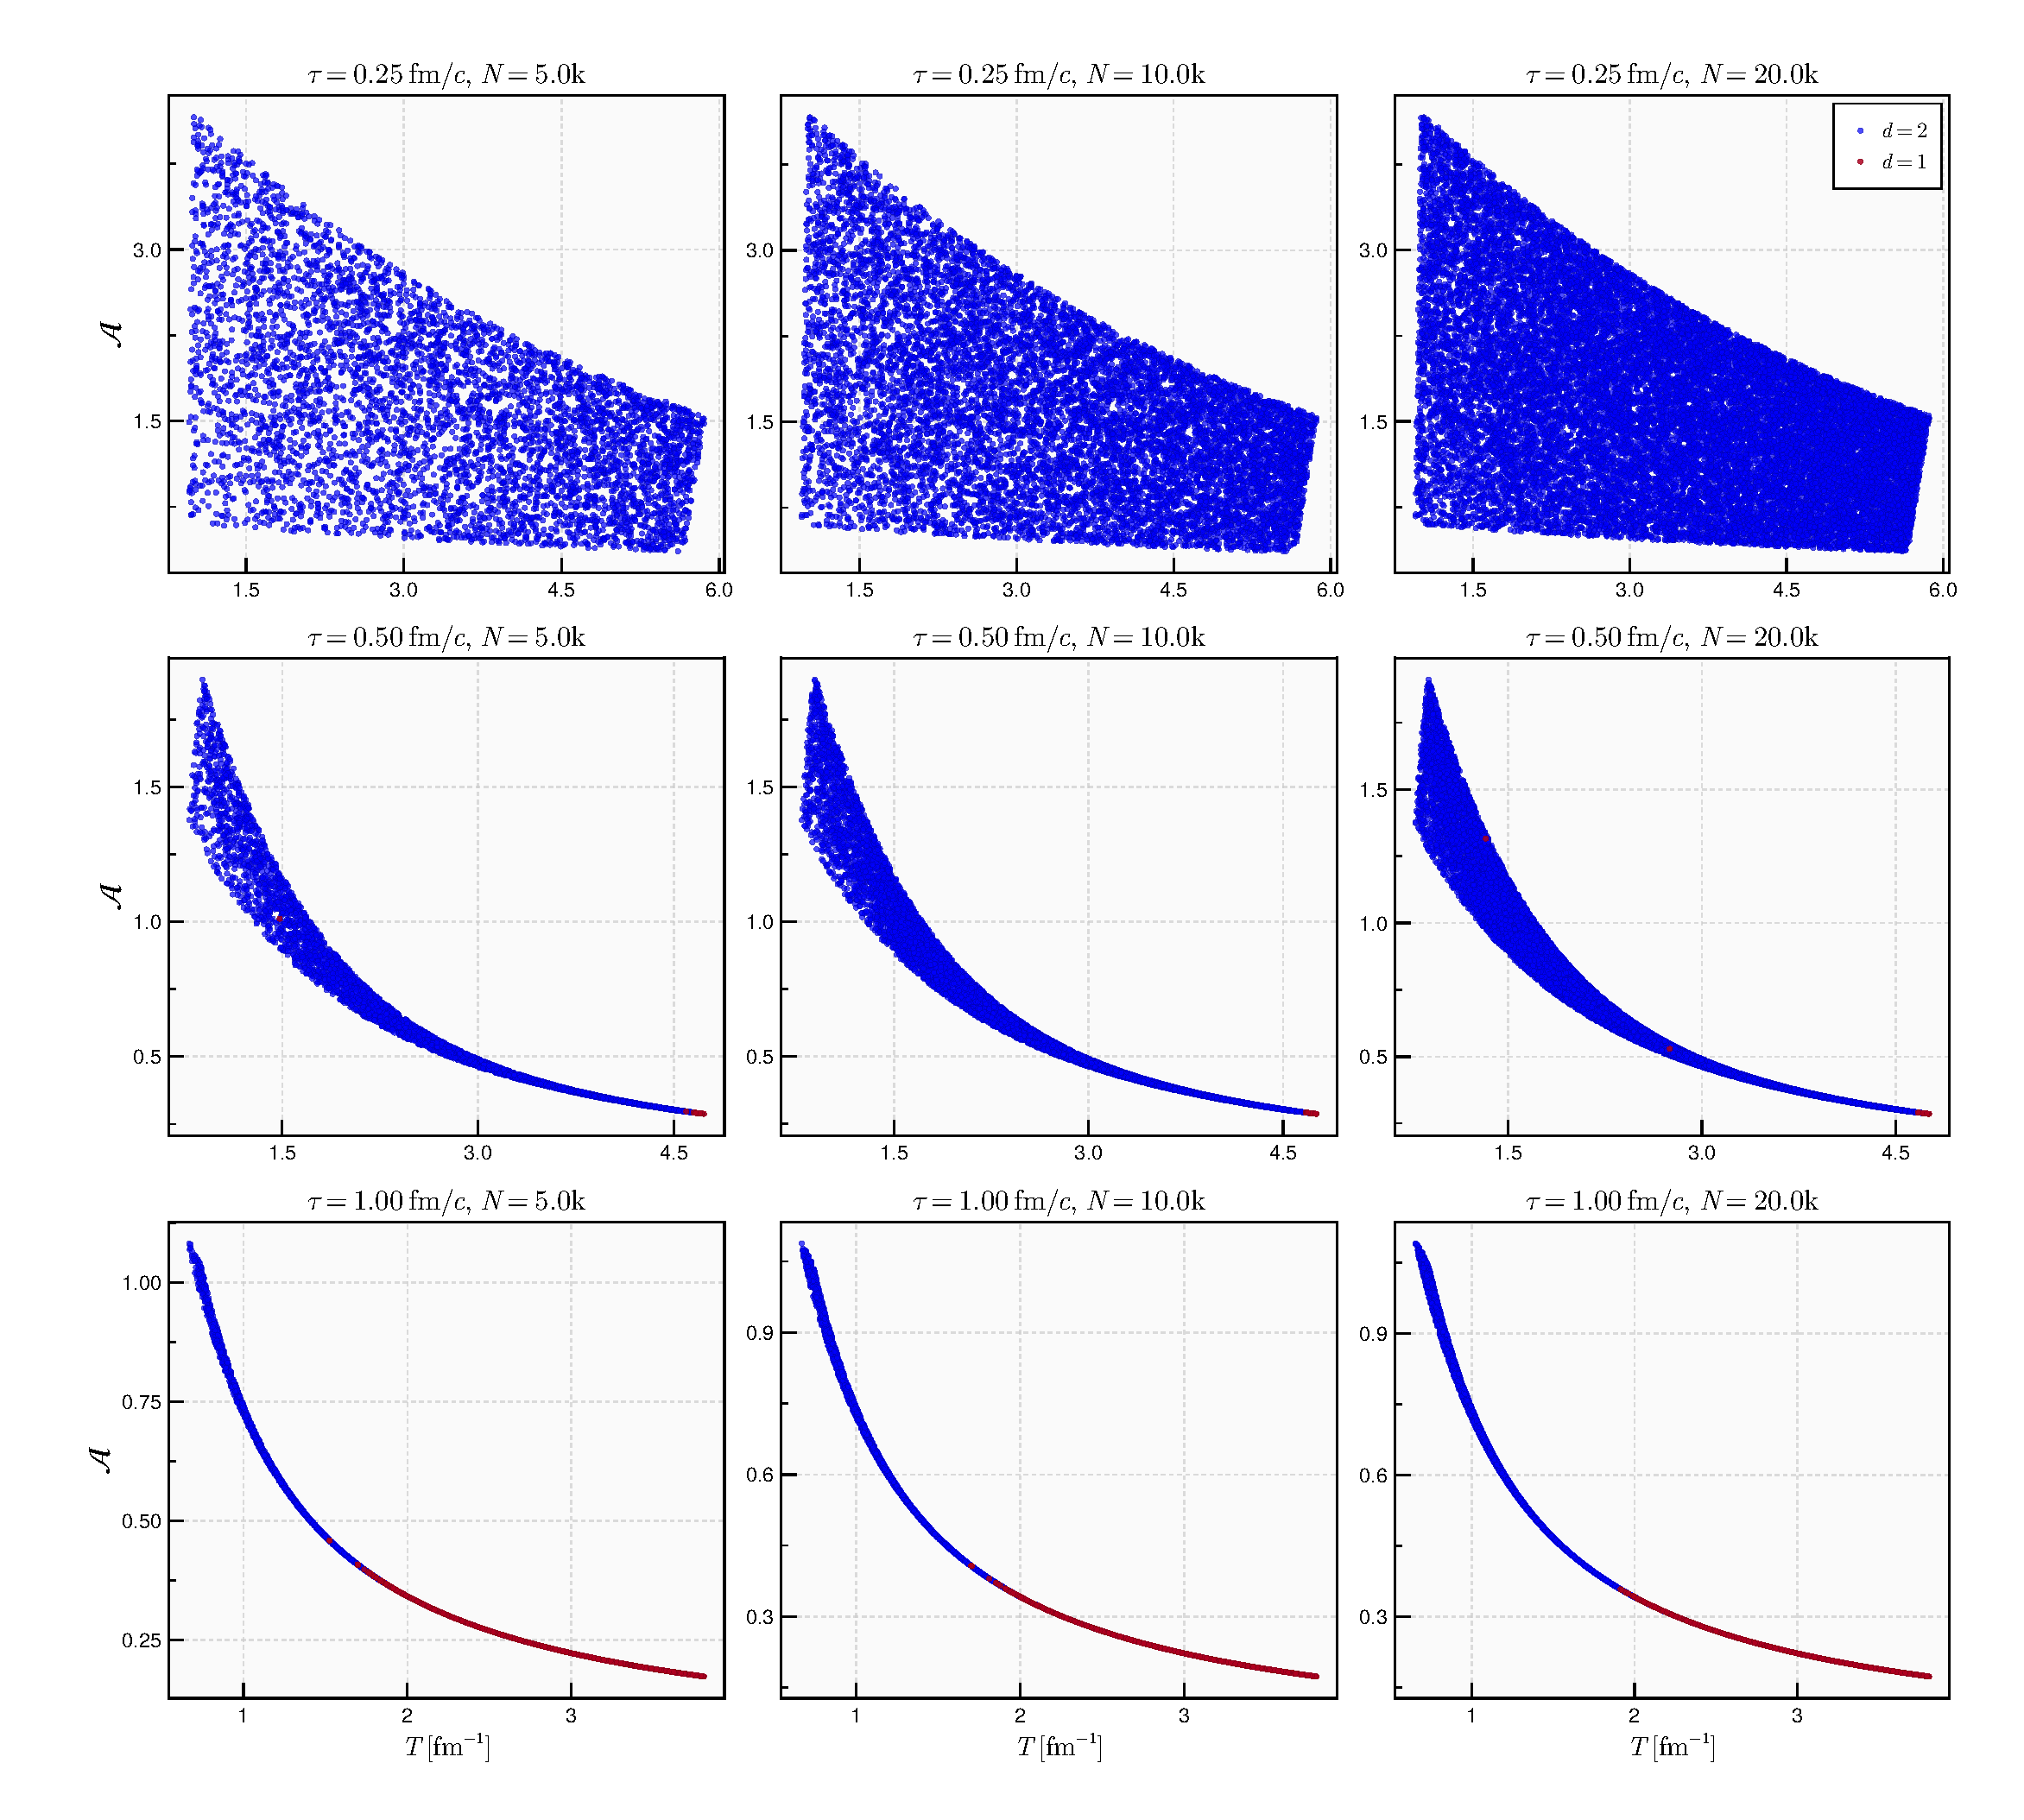
\includegraphics[width=0.92\linewidth]{sample_size_comparison/mis_phase_space_k8_sample_size_comparison.pdf}
    \caption{\textbf{The Sample Size Dilemma at Fixed $K = 8$.} Columns display increasing sample sizes ($N = 5\,000, 10\,000, 20\,000$), while rows show proper times $\tau = 0.25, 0.50, 1.00\,\mathrm{fm}/c$. As $N$ grows at fixed $K=8$, the local ball radius shrinks below the transverse bundle thickness, causing the attractor points to appear 2-dimensional (purple) even at late times $\tau = 1.00\,\mathrm{fm}/c$. This proves that $K$ must scale with $N$ according to $K_{\mathrm{opt}} \propto N^{0.45}\sqrt{D}$.}
    \label{fig:sample_size_comparison}
\end{figure}

Fig.~\ref{fig:sample_size_comparison} directly validates this phenomenon: at $K=8$, increasing $N$ to $20\,000$ suppresses the detection of the 1D attractor, retaining spurious 2D points. Only when $K$ scales adaptively to $K_{\mathrm{opt}} \approx 100$ does the true 1D universal curve emerge cleanly.

% ==============================================================================
\section{Algorithmic Specification and Data-Driven Selection}
\label{sec:algorithm}
% ==============================================================================

\begin{tcolorbox}[colback=gray!5!white,colframe=blue!75!black,title=\textbf{Algorithm 1: Adaptive Neighborhood Calibration and Local PR Dimension Estimation},fonttitle=\bfseries]
\textbf{Input:} Slice coordinates $\mathbf{X}_\tau \in \mathbb{R}^{N \times D}$ at proper time $\tau$, sample size $N$, ambient dimension $D$.\\
\textbf{Output:} Calibrated neighborhood parameter $K_{\mathrm{opt}}$ and pointwise dimensions $\mathbf{d}_{\mathrm{PR}} \in \mathbb{R}^N$.

\vspace{0.5em}
\textbf{1. Metric Standardization (Aspect-Ratio Invariance):}
\begin{itemize}
    \item Compute empirical means $\mu_k = \frac{1}{N}\sum_{i=1}^N X_{\tau, i, k}$ and standard deviations $\sigma_k = \sqrt{\frac{1}{N-1}\sum_{i=1}^N (X_{\tau, i, k} - \mu_k)^2}$.
    \item Rescale coordinates: $\tilde{X}_{\tau, i, k} \gets (X_{\tau, i, k} - \mu_k) / \sigma_k$.
\end{itemize}

\textbf{2. Analytical Anchor Evaluation:}
\begin{itemize}
    \item Compute $K_{\min} = \min(12D, \max(2, \lfloor N/2 \rfloor))$, \quad $K_{\mathrm{scale}} = \mathrm{round}(N^{0.45}\sqrt{D})$.
    \item Compute $K_{\max} = \max(K_{\min}, \min(\lfloor N/10 \rfloor, N-1))$.
    \item Analytical baseline: $K_{\mathrm{rule}} = \mathrm{clamp}(K_{\mathrm{scale}}, K_{\min}, K_{\max})$.
\end{itemize}

\textbf{3. Multi-scale Verification Grid:}
\begin{itemize}
    \item Select candidate grid $\mathcal{K} = \{K_1, \dots, K_M\}$ around $K_{\mathrm{rule}}$ (e.g., $K \in [16, 160]$).
    \item For each $K \in \mathcal{K}$:
    \begin{enumerate}
        \item Retrieve $K$ nearest neighbors $\mathcal{N}_K(\tilde{\mathbf{x}}_i)$ using KD-tree.
        \item Construct local covariance: $\mathbf{C}_i(K) = \frac{1}{K-1}\sum_{j \in \mathcal{N}_K} (\tilde{\mathbf{x}}_j - \bar{\mathbf{x}}_i)(\tilde{\mathbf{x}}_j - \bar{\mathbf{x}}_i)^T$.
        \item Compute $d_{\mathrm{PR}}(\tilde{\mathbf{x}}_i; K) = (\mathrm{Tr}\,\mathbf{C}_i)^2 / \mathrm{Tr}(\mathbf{C}_i^2)$.
        \item Calculate Sarle's bimodality coefficient \cite{Sarle1983}: $b(K) = (\gamma^2 + 1)/\kappa$, where $\gamma = \mathrm{skew}(\mathbf{d}_{\mathrm{PR}})$, $\kappa = \mathrm{kurt}(\mathbf{d}_{\mathrm{PR}})$.
        \item Calculate scale sensitivity: $S(K) = |\partial \langle d_{\mathrm{PR}} \rangle / \partial \log K|$.
    \end{enumerate}
\end{itemize}

\textbf{4. Optimal Scale Selection:}
\begin{itemize}
    \item \textbf{If} $\max_{K} b(K) > 0.60$: \textbf{return} $K_{\mathrm{opt}} = \arg\max_{K} b(K)$ \hfill (Transient Relaxation Regime)
    \item \textbf{Else}: \textbf{return} $K_{\mathrm{opt}} = \arg\min_{K} S(K)$ \hfill (Scale-Invariance Plateau)
\end{itemize}
\end{tcolorbox}

% ==============================================================================
\section{Numerical Verification and Multiscale Diagnostics}
\label{sec:numerical_results}
% ==============================================================================
To verify the validity of Eq.~(\ref{eq:k_opt_formula}), we analyze the full ensemble of $N = 20\,000$ conformal MIS trajectories. In Table~\ref{tab:mis_stages_table}, we present the statistical evolution of $d_{\mathrm{PR}}$ across proper time $\tau$ under $K = 100$.

\begin{table}[htbp]
    \centering
    \caption{Evolution of local participation ratio dimension across proper time $\tau$ for MIS ($N = 20\,000$, $K_{\mathrm{opt}} = 100$).}
    \label{tab:mis_stages_table}
    \vspace{0.4em}
    \begin{tabular}{@{}l c c c c l@{}}
        \toprule
        $\tau\,[\mathrm{fm}/c]$ & $\langle d_{\mathrm{PR}} \rangle$ & $\sigma(d_{\mathrm{PR}})$ & $f_{1\mathrm{D}}\,(<1.3)$ & $f_{2\mathrm{D}}\,(>1.7)$ & \textbf{Hydrodynamic Stage} \\
        \midrule
        $0.20$ & $1.94$ & $0.09$ & $0.0\%$ & $95.1\%$ & Stage 1: Expansion (pure 2D) \\
        $0.25$ & $1.94$ & $0.10$ & $0.0\%$ & $93.8\%$ & Stage 1: Expansion (pure 2D) \\
        $0.35$ & $1.89$ & $0.15$ & $0.3\%$ & $85.7\%$ & Stage 1: Expansion (pure 2D) \\
        \midrule
        $0.45$ & $1.73$ & $0.28$ & $13.1\%$ & $60.8\%$ & Stage 2: Mode Damping (Onset) \\
        $0.55$ & $1.48$ & $0.39$ & $41.9\%$ & $37.3\%$ & Stage 2: Mode Damping (Bimodal) \\
        $0.65$ & $1.33$ & $0.38$ & $59.9\%$ & $24.6\%$ & Stage 2: Mode Damping (Attractor core) \\
        \midrule
        $0.80$ & $1.19$ & $0.31$ & $75.4\%$ & $12.0\%$ & Stage 3: Attractor Evolution \\
        $1.00$ & $1.07$ & $0.16$ & $90.3\%$ & $1.0\%$ & Stage 3: Universal Attractor \\
        $2.50$ & $1.00$ & $0.00$ & $100.0\%$ & $0.0\%$ & Stage 3: Universal Attractor \\
        \bottomrule
    \end{tabular}
\end{table}

\begin{figure}[htbp]
    \centering
    \begin{subfigure}[b]{0.49\textwidth}
        \centering
        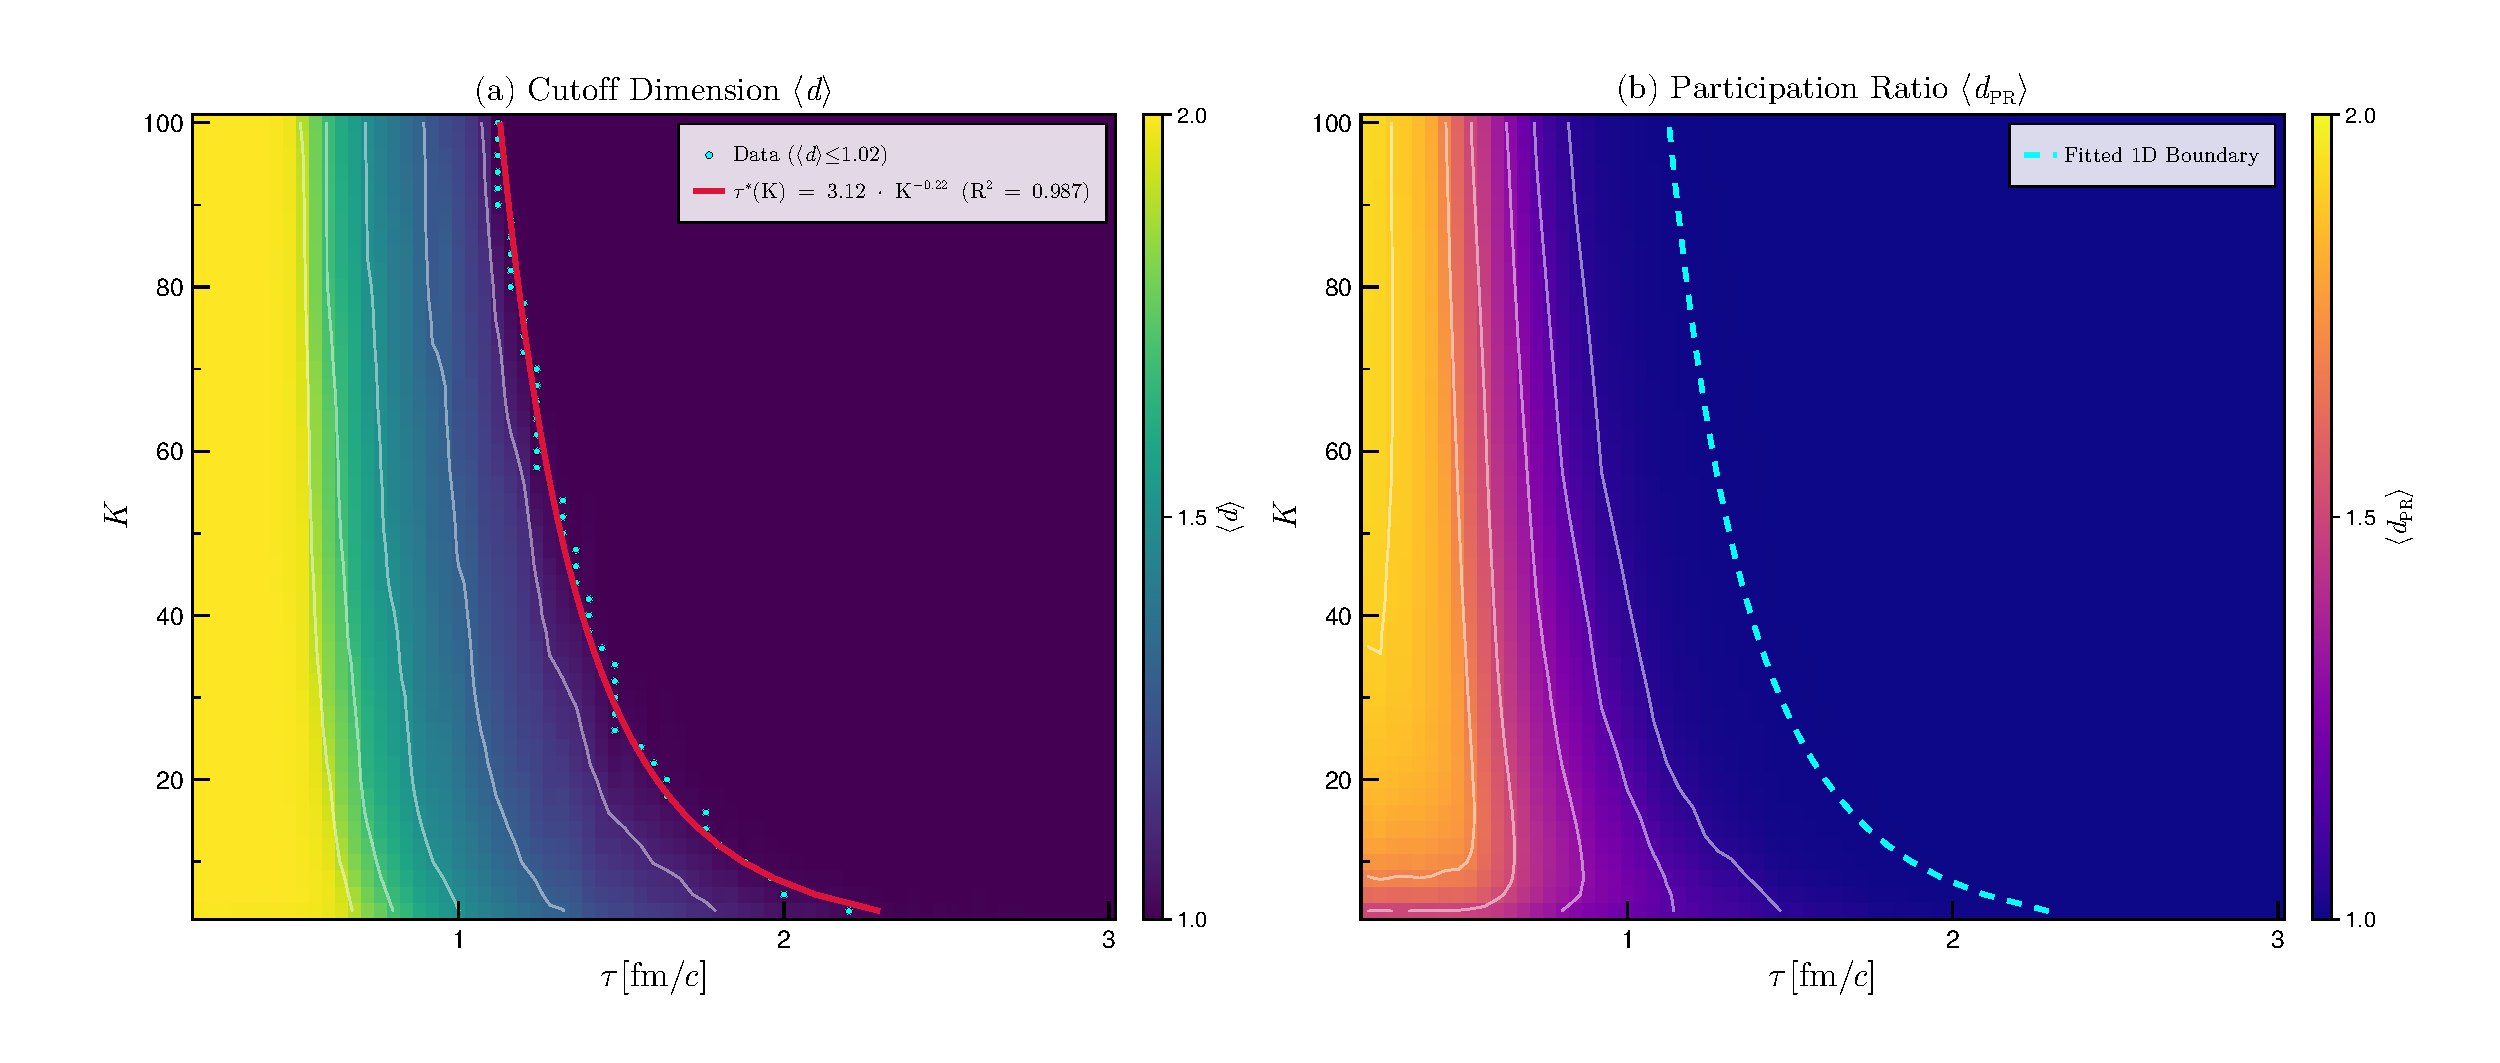
\includegraphics[width=\linewidth]{dimension_map/map_mean_dimension_tau_vs_k_dual.pdf}
        \caption{Continuous parameter map $\langle d \rangle(\tau, K)$ and fitted collapse threshold $\tau^*(K)$.}
        \label{fig:map_dimension_dual}
    \end{subfigure}
    \hfill
    \begin{subfigure}[b]{0.49\textwidth}
        \centering
        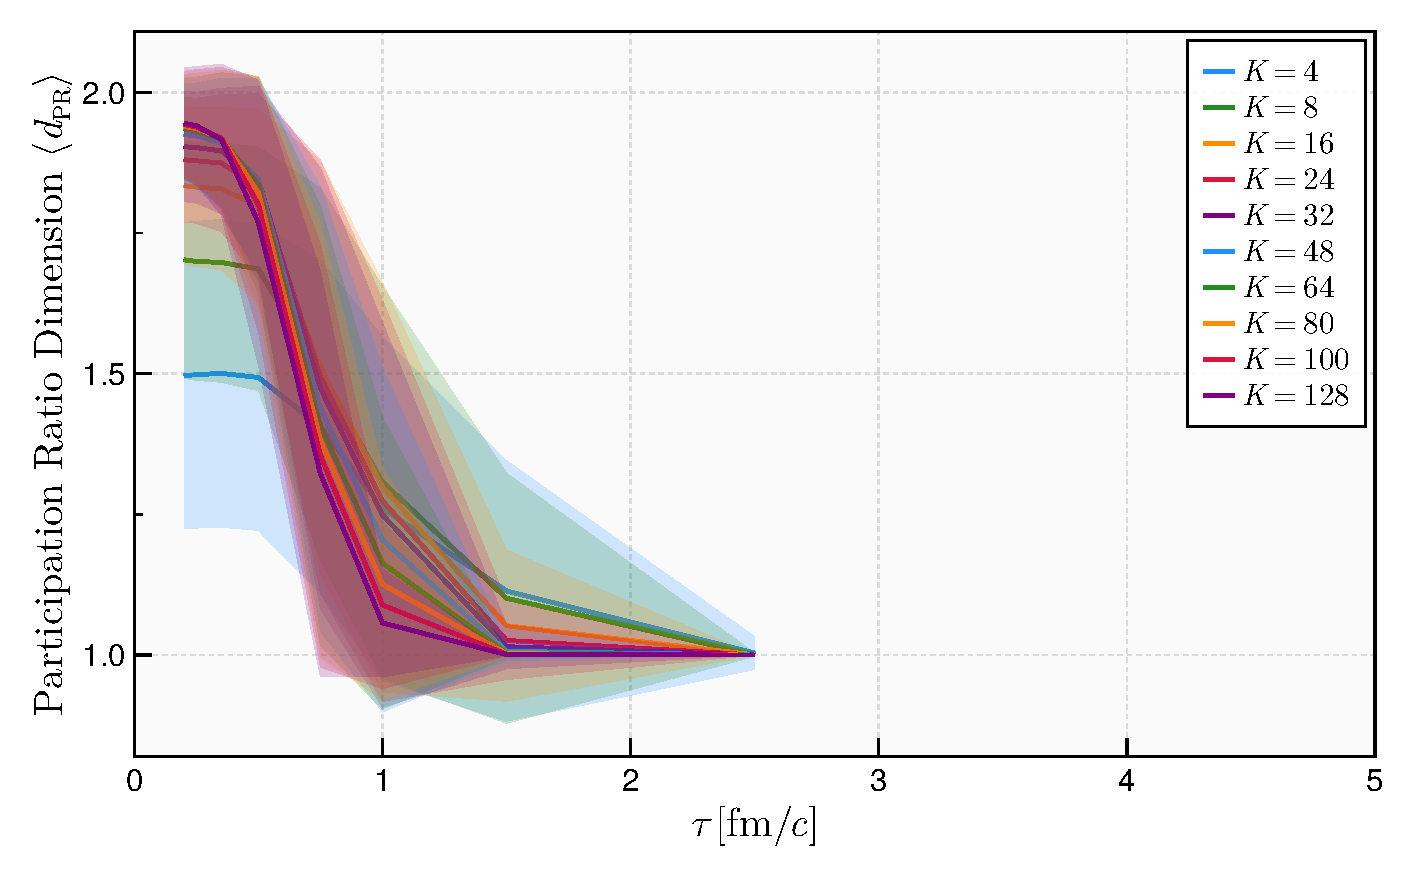
\includegraphics[width=\linewidth]{k_dependency/k_sweep_mis_physical_coordinates_TA_pr.pdf}
        \caption{Multiscale $K$-dependency curves $\langle d_{\mathrm{PR}} \rangle(\tau)$.}
        \label{fig:k_bands}
    \end{subfigure}
    \caption{\textbf{Multiscale $K$-scale diagnostics.} (a) Continuous 2D heatmap of local dimension $\langle d \rangle$ across proper time $\tau$ and neighborhood size $K$, alongside the fitted collapse threshold $\tau^*(K) \approx a \cdot K^b$. (b) Trajectory dimension curves $\langle d_{\mathrm{PR}} \rangle$ across scale pairs $(K, 2K)$ with $\pm 1\sigma$ uncertainty bands, demonstrating that scale sensitivity $|\Delta d| \to 0$ vanishes near $K_{\mathrm{opt}} \approx 100$.}
    \label{fig:multiscale_diagnostics}
\end{figure}

The diagnostics in Fig.~\ref{fig:multiscale_diagnostics} provide direct evidence of the mechanism:
\begin{itemize}
    \item In Fig.~\ref{fig:map_dimension_dual}, the continuous $(\tau, K)$ heatmap displays a broad horizontal plateau for $K \ge 64$. The fitted collapse boundary follows a clean power-law scaling $\tau^*(K) \sim K^b$, demonstrating the smooth dependence of the observable transition on neighborhood scale.
    \item In Fig.~\ref{fig:k_bands}, the discrepancy between $K$ and $2K$ contracts to less than $0.05$ units of dimension around $K \approx 100$.
    \item At $\tau = 0.55\,\mathrm{fm}/c$, Sarle's bimodality coefficient reaches $b \approx 0.75 \gg 5/9$, demonstrating that the distribution split into two distinct sub-populations is a physical reality rather than a numerical artifact.
\end{itemize}

% ==============================================================================
\section{Generalization to 3D Phase Space (HJSW Model)}
\label{sec:hjsw_generalization}
% ==============================================================================
To test the generality of our heuristic in higher-dimensional embeddings, we evaluate the Heller--Janik--Spaliński--Witaszczyk (HJSW) model, where the dynamical variables span a 3-dimensional phase space $(T, \mathcal{A}, \mathcal{B})$ ($D=3$). For $N = 10\,000$, Eq.~(\ref{eq:k_opt_formula}) dictates $K_{\mathrm{opt}} \approx 109$.

\begin{figure}[htbp]
    \centering
    \begin{subfigure}[b]{0.49\textwidth}
        \centering
        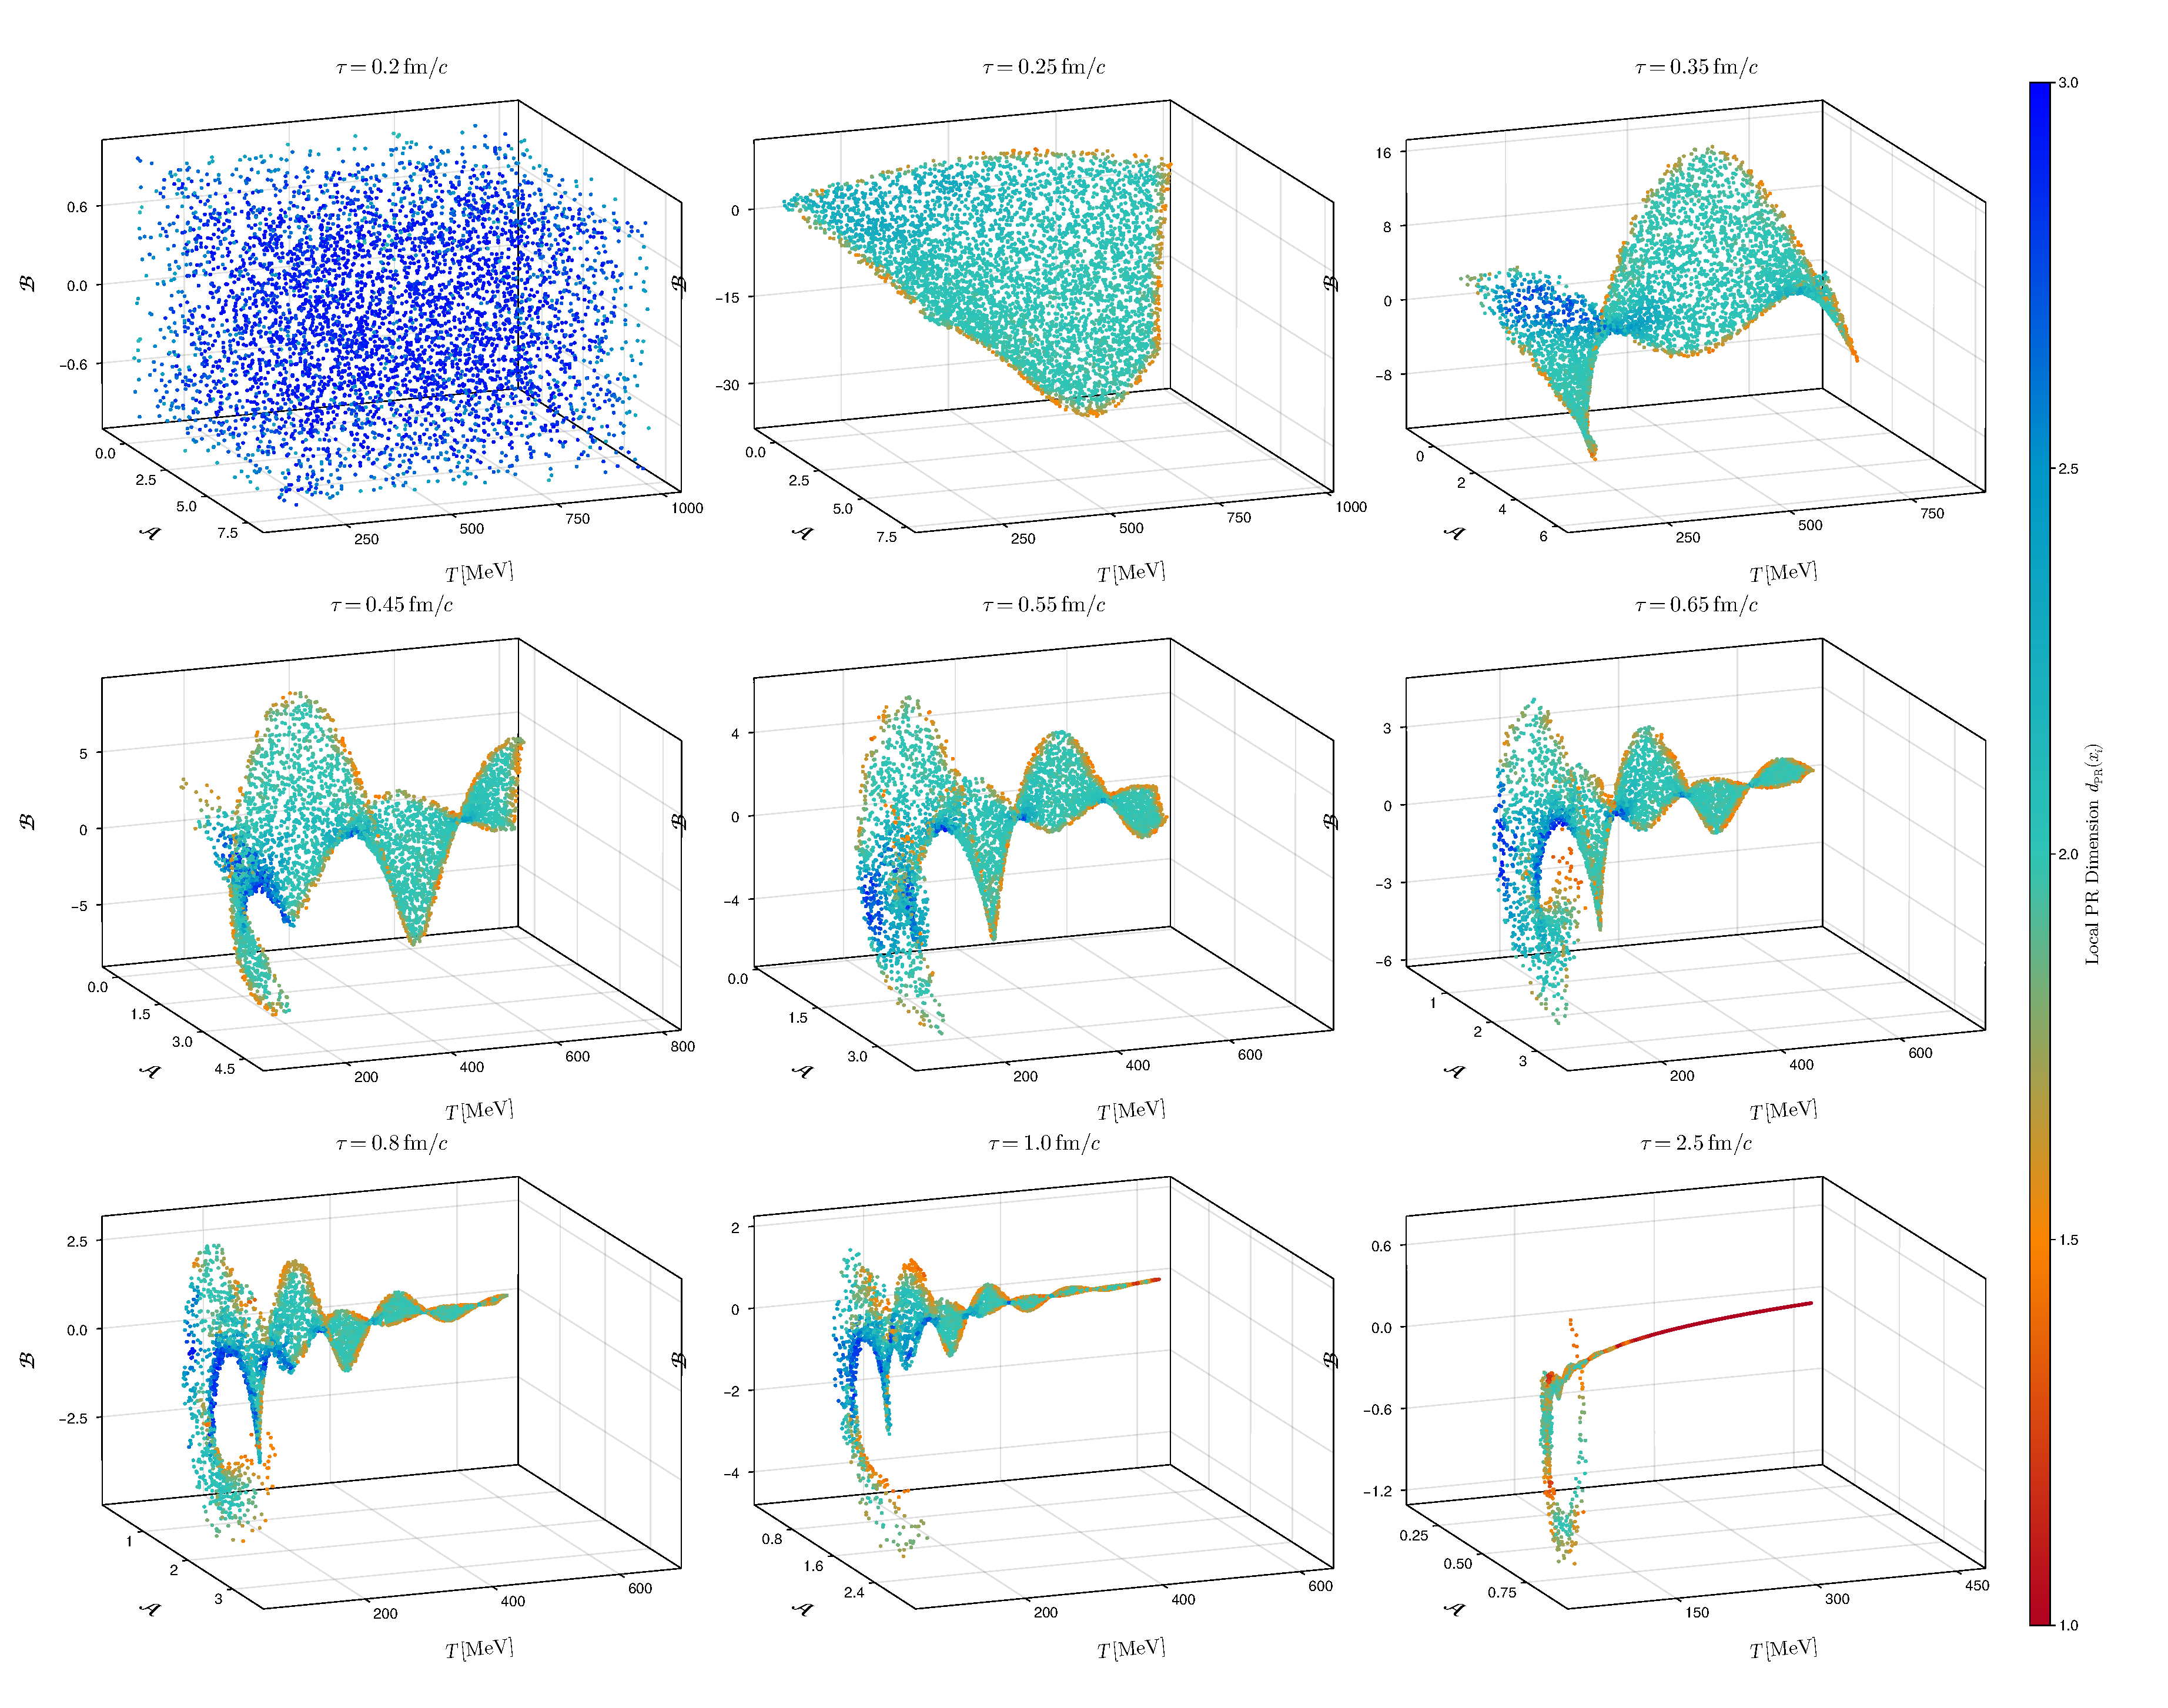
\includegraphics[width=\linewidth]{phase_space/hjsw/grid_hjsw_physical_pr.pdf}
        \caption{3D Phase Space in physical units ($T\,[\mathrm{MeV}], \mathcal{A}, \mathcal{B}$).}
        \label{fig:hjsw_phase_space}
    \end{subfigure}
    \hfill
    \begin{subfigure}[b]{0.49\textwidth}
        \centering
        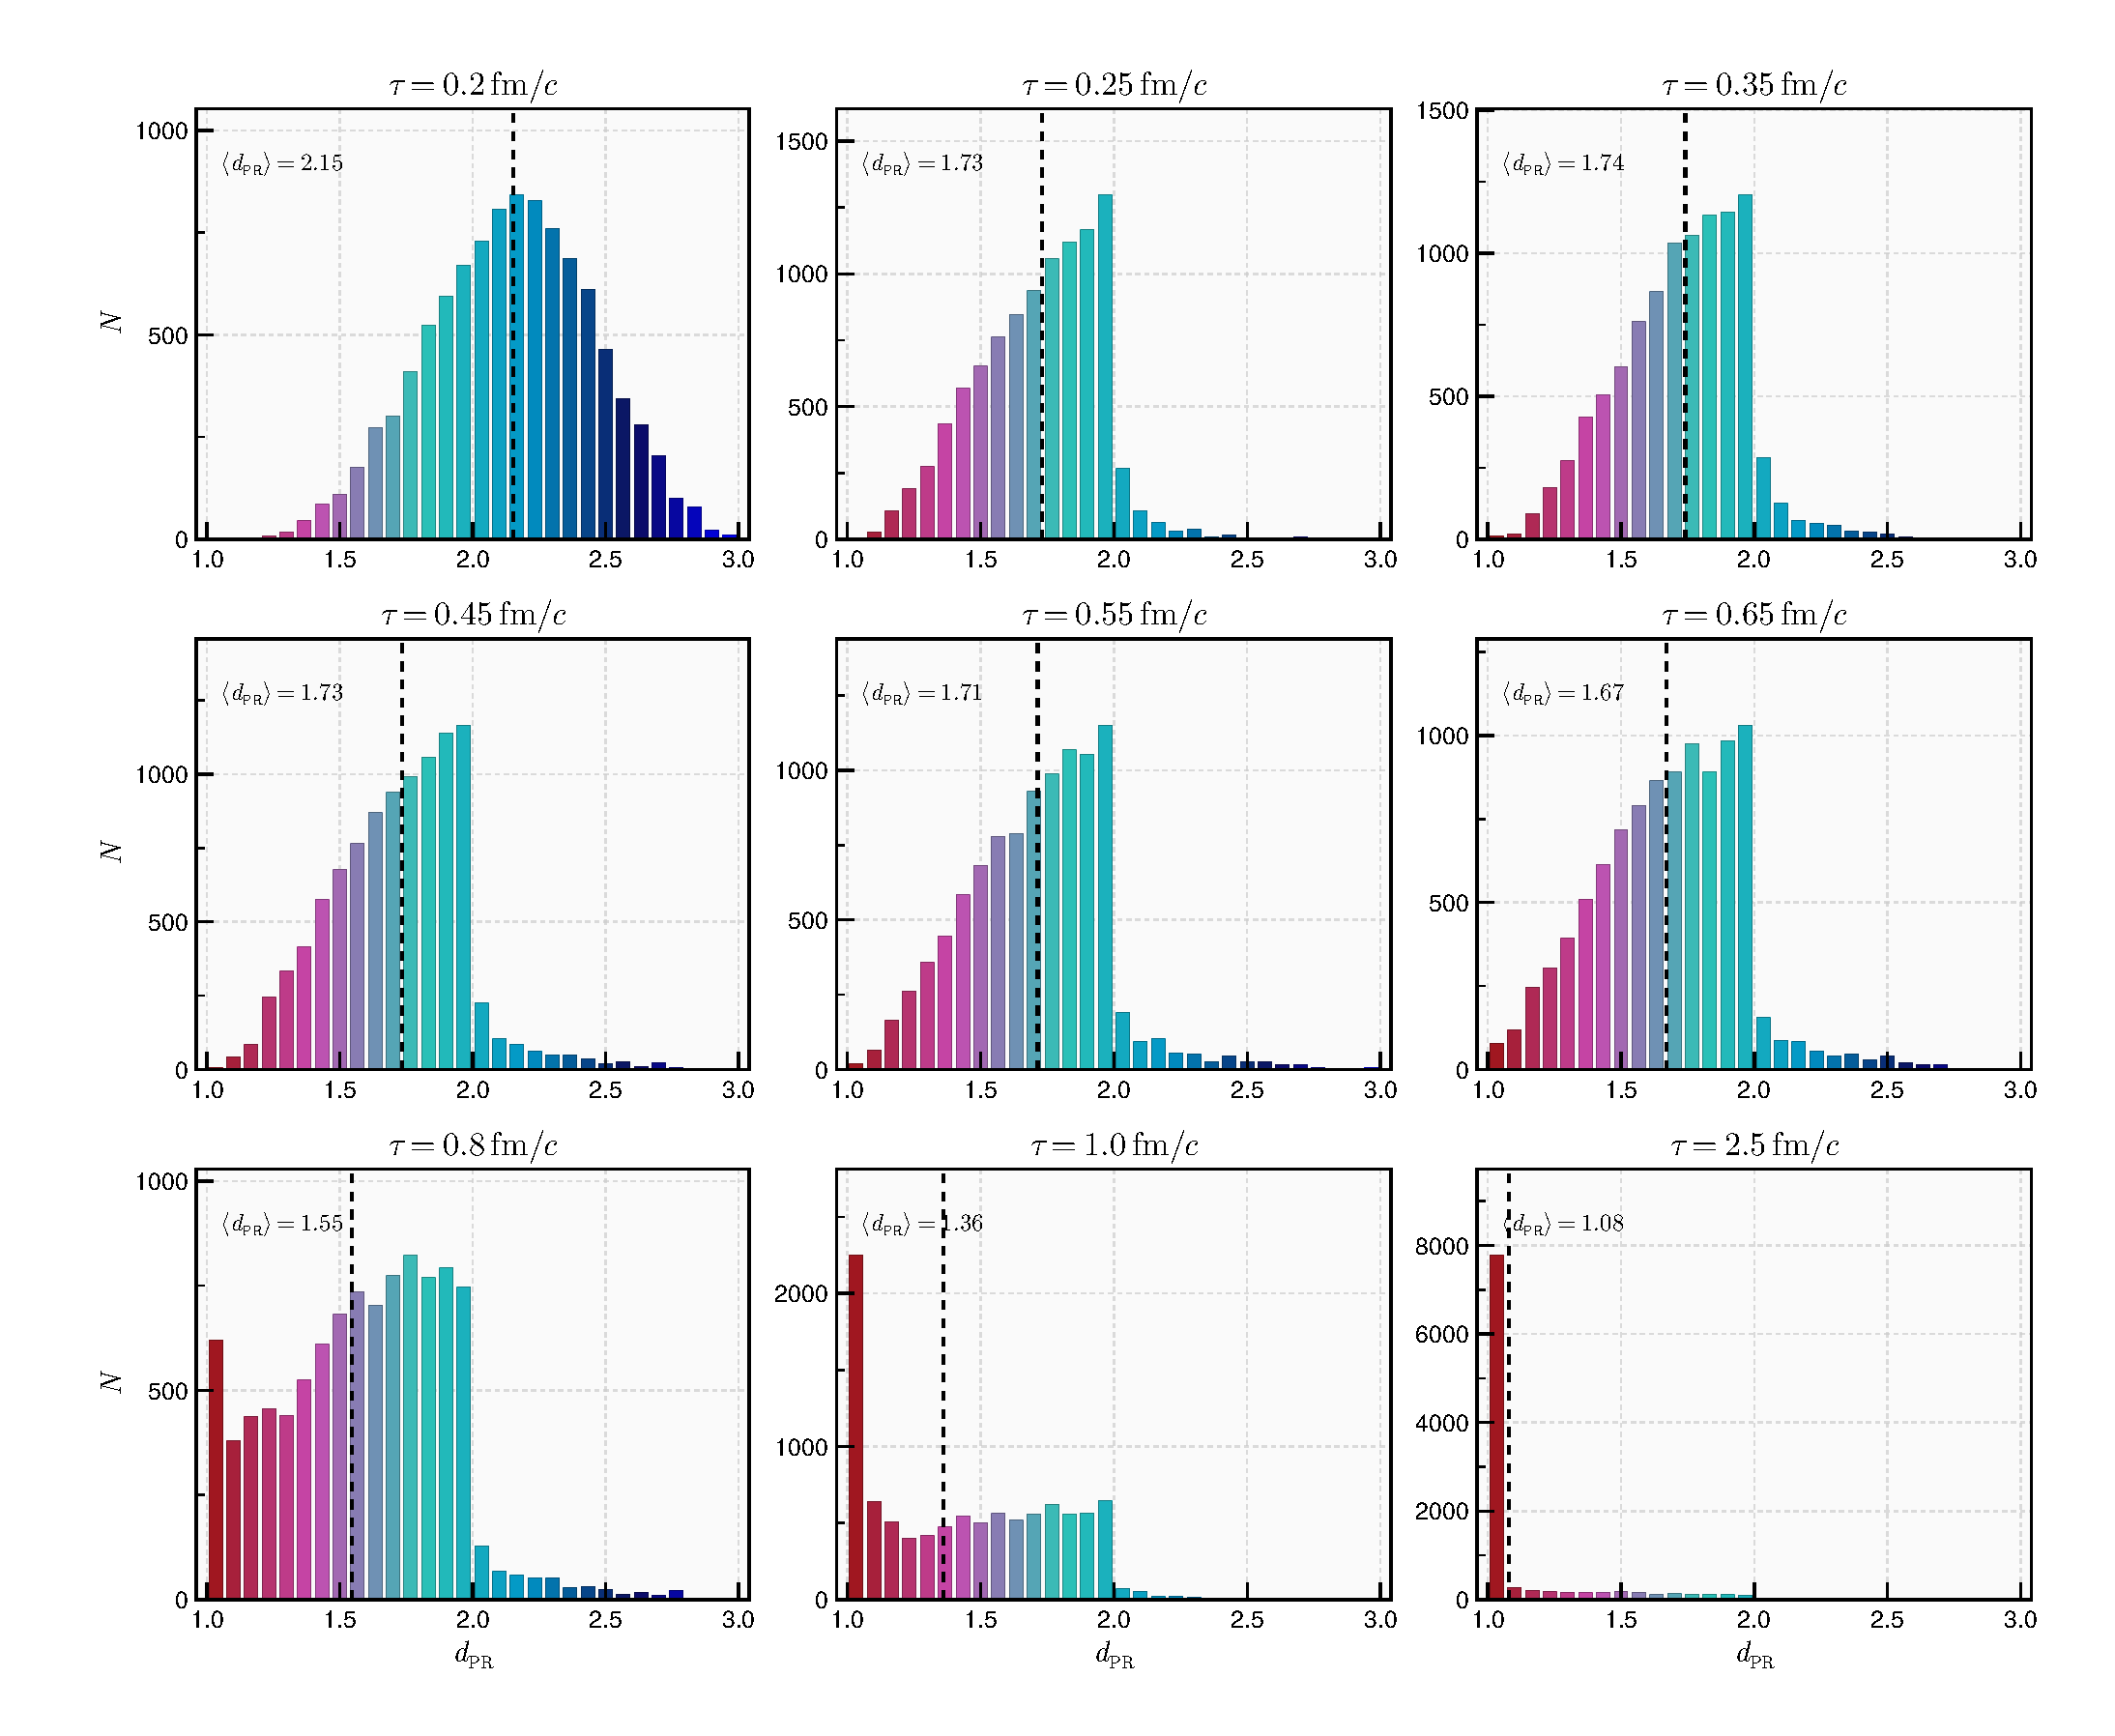
\includegraphics[width=\linewidth]{phase_space/hjsw/grid_hjsw_physical_pr_hist.pdf}
        \caption{Stacked histograms of $d_{\mathrm{PR}}$ (binned by initial $\mathcal{A}$).}
        \label{fig:hjsw_histograms}
    \end{subfigure}
    \caption{\textbf{Hydrodynamic collapse in the 3D HJSW Model in physical units ($K = 100$).} (a) 3D phase-space trajectory cloud displaying physical coordinates on all axes ($T \in [100, 1000]\,\mathrm{MeV}$, $\mathcal{A} \in [-1, 2.5]$, $\mathcal{B} \in [-1, 1]$), with points colored by the local PR dimension $d_{\mathrm{PR}}$ computed via $Z$-score standardized local PCA ($K = 100$). (b) Stacked histograms of local dimension $d_{\mathrm{PR}}$ demonstrating the two-stage collapse: the 3D volume at $\tau = 0.20\,\mathrm{fm}/c$ ($\langle d_{\mathrm{PR}} \rangle = 2.82 \pm 0.17$, $94.2\%$ with $d_{\mathrm{PR}} > 2.5$) contracts rapidly as the fast non-hydrodynamic mode $\mathcal{B}$ decays into an intermediate 2D sheet ($d \approx 2.0$) at $\tau = 0.25\,\mathrm{fm}/c$, before collapsing toward the 1D hydrodynamic attractor ($d \to 1.0$) at late times.}
    \label{fig:hjsw_overview}
\end{figure}

As exhibited in Fig.~\ref{fig:hjsw_overview}, the 3D ensemble initiates at $d \approx 3.0$ during early expansion ($\tau \le 0.35\,\mathrm{fm}/c$). During the transient regime ($\tau \sim 0.55\,\mathrm{fm}/c$), solutions rapidly decay through an intermediate 2D sheet before collapsing onto the one-dimensional hydrodynamical attractor ($d \to 1.0$).

% ==============================================================================
\section{Conclusion and Practical Recommendations}
\label{sec:conclusion}
% ==============================================================================
We have resolved the open problem of neighborhood calibration and coordinate metric distortion in local dimension analysis of hydrodynamic attractors. The primary conclusions and practical guidelines for practitioners are:

\begin{enumerate}
    \item \textbf{The One-Shot Plug-and-Play Rule for $K$:} Compute $K$ once at the beginning of the analysis from the known dataset size $N$ and ambient dimension $D$:
    \begin{equation}
        \boxed{K = \mathrm{clamp}\left(\mathrm{round}\left(N^{0.45}\sqrt{D}\right), \; 12D, \; \left\lfloor\frac{N}{10}\right\rfloor\right)}
    \end{equation}
    For standard publication ensembles ($N = 10\,000$--$20\,000$), this prescribes setting:
    \begin{itemize}
        \item \textbf{Conformal MIS ($D=2$):} $K = 100$ (or $K \approx 1.41 \cdot N^{0.45}$).
        \item \textbf{HJSW Model ($D=3$):} $K = 100$--$110$ (or $K \approx 1.73 \cdot N^{0.45}$).
    \end{itemize}
    This single $K$ is set globally at the start and kept constant across all proper time slices $\tau \in [0.20, 2.50]\,\mathrm{fm}/c$ without any per-slice retuning.
    \item \textbf{Always standardize coordinates ($Z$-score):} Never perform nearest-neighbor searches in raw physical coordinates where temperature dominates over anisotropy. Standardization acts as an empirical diagonal Mahalanobis metric, rendering local PCA invariant under scale and chart dilations.
    \item \textbf{A Posteriori Validation (Sanity Check):} Multi-scale bimodality ($b(K) > 0.60$) and scale plateaus ($|\Delta d / \Delta \log K| \approx 0$) serve as optional confirmation that this single global choice of $K$ reliably separates the attractor core from the transient wings.
\end{enumerate}

\begin{thebibliography}{99}
\bibitem{BickelLevina2005}
E.~Levina and P.~J.~Bickel,
\emph{Maximum Likelihood Estimation of Intrinsic Dimension},
Adv. Neural Inf. Process. Syst. \textbf{17}, 777--784 (2005).
\href{https://proceedings.neurips.cc/paper_files/paper/2004/hash/74fbc16c530eb106688f1acbcb44fbee-Abstract.html}{[NeurIPS]}
\href{https://www.stat.berkeley.edu/~bickel/mldim.pdf}{[PDF]}

\bibitem{LittleMaggioni2009}
A.~V.~Little, M.~Maggioni, and L.~Rosasco,
\emph{Multiscale Geometric Methods for Data Sets I: Multiscale SVD, Noise and Curvature},
Appl. Comput. Harmon. Anal. \textbf{43}, 504--567 (2017).
\href{https://doi.org/10.1016/j.acha.2015.09.009}{doi:10.1016/j.acha.2015.09.009},
\href{https://arxiv.org/abs/1202.2687}{arXiv:1202.2687 [math.ST]};
preliminary version in \emph{Proc. 2009 IEEE Workshop on Statistical Signal Processing}, 477 (2009),
\href{https://doi.org/10.1109/SSP.2009.5278546}{doi:10.1109/SSP.2009.5278546}.

\bibitem{Heller2015}
M.~P.~Heller and M.~Spali\'nski,
\emph{Hydrodynamics Beyond the Gradient Expansion: Resurgence and Attractors},
Phys. Rev. Lett. \textbf{115}, 072501 (2015).
\href{https://doi.org/10.1103/PhysRevLett.115.072501}{doi:10.1103/PhysRevLett.115.072501},
\href{https://arxiv.org/abs/1503.07514}{arXiv:1503.07514 [hep-th]}.

\bibitem{MarchenkoPastur1967}
V.~A.~Marchenko and L.~A.~Pastur,
\emph{Distribution of Eigenvalues for Some Sets of Random Matrices},
Math. USSR-Sb. \textbf{1}, 457--483 (1967) [Mat. Sb. \textbf{72}(114), 507 (1967)].
\href{https://doi.org/10.1070/SM1967v001n04ABEH001994}{doi:10.1070/SM1967v001n04ABEH001994}.

\bibitem{Heller2014}
M.~P.~Heller, R.~A.~Janik, M.~Spali\'nski, and P.~Witaszczyk,
\emph{Coupling Hydrodynamics to Nonequilibrium Degrees of Freedom in Strongly Coupled Plasmas},
Phys. Rev. Lett. \textbf{113}, 261601 (2014).
\href{https://doi.org/10.1103/PhysRevLett.113.261601}{doi:10.1103/PhysRevLett.113.261601},
\href{https://arxiv.org/abs/1409.5087}{arXiv:1409.5087 [hep-th]}.

\bibitem{Romatschke2017}
P.~Romatschke,
\emph{Relativistic Fluid Dynamics Far From Local Equilibrium},
Phys. Rev. Lett. \textbf{120}, 012301 (2018).
\href{https://doi.org/10.1103/PhysRevLett.120.012301}{doi:10.1103/PhysRevLett.120.012301},
\href{https://arxiv.org/abs/1704.08699}{arXiv:1704.08699 [nucl-th]}.

\bibitem{Spalinski2016}
M.~Spali\'nski,
\emph{On the Hydrodynamic Attractor of a System of Particles in One-Dimensional Expansion},
Phys. Lett. B \textbf{776}, 468--472 (2018).
\href{https://doi.org/10.1016/j.physletb.2017.11.059}{doi:10.1016/j.physletb.2017.11.059},
\href{https://arxiv.org/abs/1708.01921}{arXiv:1708.01921 [hep-th]}.

\bibitem{Sarle1983}
W.~S.~Sarle,
\emph{The Multimodality and Bimodality of Distributions},
SAS Technical Report A-107, SAS Institute Inc., Cary, NC (1983).
\href{https://support.sas.com/documentation/onlinedoc/stat/141/multivar.pdf}{[SAS Documentation]}.

\bibitem{Campadelli2015}
P.~Campadelli, E.~Casiraghi, C.~Ceruti, and A.~Rozza,
\emph{Intrinsic Dimension Estimation: Relevant Techniques and a Benchmark Framework},
Math. Probl. Eng. \textbf{2015}, 759519 (2015).
\href{https://doi.org/10.1155/2015/759519}{doi:10.1155/2015/759519}.
\end{thebibliography}

\end{document}
